\documentclass{beamer}
\usepackage{graphicx} % Required for inserting images
\usepackage{tikz}
\usepackage{geometry}
\usepackage{amsmath}
\usepackage{algorithm}
\usepackage{algpseudocode}
\usepackage{amsfonts}
\usepackage{caption}
\usepackage{xcolor}

\usepackage[none]{hyphenat}

\usetheme{Madrid}
\usecolortheme{seahorse}

\geometry{bottom=0in}

\title{Boundary Area}
\author{Saha Kuljit Shantanu}
\date{1905119}

\begin{document}



\maketitle

\section{We need to know}



\begin{frame}{We need to know}

\begin{block}{Handling Boundary edges}
   When partitioning a problem space (\textbf{such as a geometric space or a graph}), the elements near the \textbf{boundaries of partitions} may interact with elements in neighboring partitions. These interactions can create \textbf{edge effects}, where the behavior near the boundary is different from that in the interior.
\end{block}
    
    % Block 2: Unit Disk Graph
\begin{block}{Decomposing Global Problems}
    For some problems, the \textbf{global structure} is more important than the local details. By studying the boundaries, you can better understand how to decompose the global problem into manageable subproblems \textbf{without losing essential connections} or interactions between different parts of the problem.
\end{block}

\end{frame}

\begin{frame}{We need to know}

\begin{block}{Dominating Set}
    A dominating set for a graph \( G = (V, E) \) is a subset \( D \subseteq V \) such that every vertex not in \( D \) is adjacent to at least one vertex in \( D \).
\end{block}
    
    % Block 2: Unit Disk Graph
\begin{block}{Unit Disk Graph}
    A unit disk graph is a graph where each vertex represents a disk of unit diameter in the Euclidean plane. There is an edge between two points u and v if and only if the two unit disks centered at u and v have a nonempty intersection.
\end{block}
    
    % Block 3: CDS-UDG Problem
\begin{block}{CDS-UDG Problem}
    The Connected Dominating Set (CDS) problem in Unit Disk Graphs (UDGs) is to find a connected dominating set with minimum cardinality for the graph.

    %, ensuring that every node in the graph is either in the set or adjacent to a node in the set.
\end{block}

\end{frame}

\begin{frame}{UDC$_1$ visualization for $m \times m$ grid}

\begin{center}
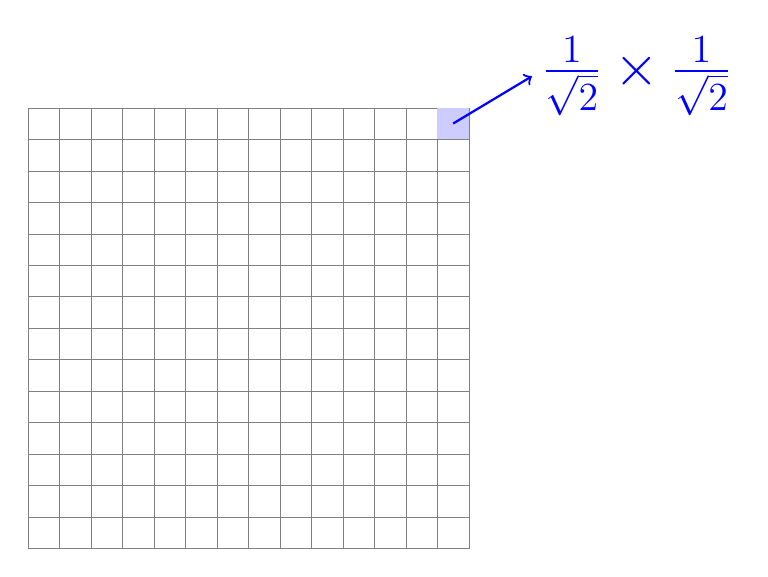
\begin{tikzpicture}[scale=0.4] % Adjust scale to fit the grid
    % Draw 14x14 grid
    \draw[step=1cm,gray,very thin] (0,0) grid (14,14);
    
    % Highlight the top-right square in blue
    \fill[blue!20] (13,13) rectangle (14,14);

    % Draw the label and arrow for 1/sqrt(2)
    \draw[blue, ->, thick] (13.5, 13.5) -- (16, 15) node[right] {\textbf{\textit{\huge $\frac{1}{\sqrt{2}} \times \frac{1}{\sqrt{2}}$}}};

\end{tikzpicture}
\end{center}

\end{frame}

\begin{frame}{UDC$_1$ visualization for $m \times m$ grid}

\begin{center}
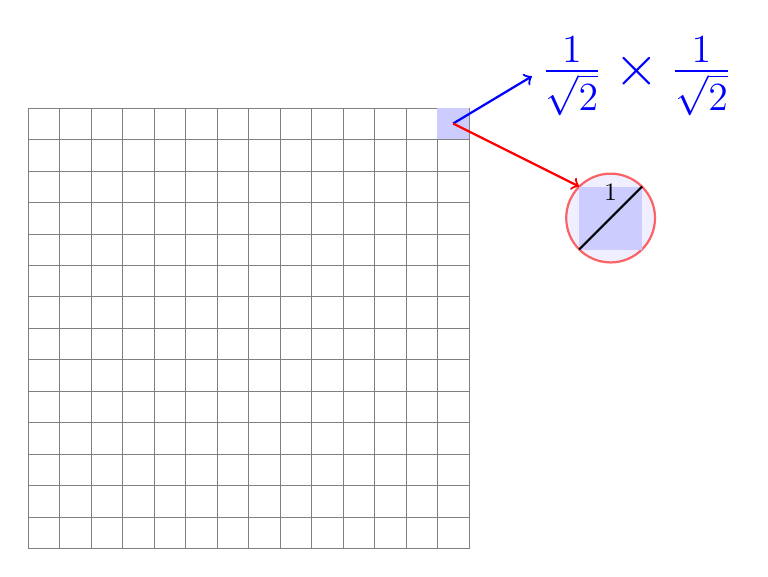
\begin{tikzpicture}[scale=0.4]
    % Draw 14x14 grid
    \draw[step=1cm,gray,very thin] (0,0) grid (14,14);
    
    % Highlight the top-right square in blue
    \fill[blue!20] (13,13) rectangle (14,14);

    \draw[blue, ->, thick] (13.5, 13.5) -- (16, 15) node[right] {\textbf{\textit{\huge $\frac{1}{\sqrt{2}} \times \frac{1}{\sqrt{2}}$}}};

    % Arrow pointing 45 degrees down-right, ending at the circumference of the circle
    

    % Draw the circumscribed circle
    \draw[red, thick, fill=blue!10, opacity=0.6] (18.5, 10.5) circle (1.41cm);

    % Large square inside the circle
    \fill[blue!20] (17.5,9.5) rectangle (19.5,11.5);

    % Label the diameter of the circle as 1
    \draw[thick] (17.5, 9.5) -- (19.5, 11.5); % Diameter line
    \node at (18.5, 11.3) {\small $1$}; % Label for the diameter

    \draw[red, ->, thick] (13.5, 13.5) -- (17.5, 11.5);
\end{tikzpicture}
\end{center}

\end{frame}

\begin{frame}{UDC$_1$ visualization for $m \times m$ grid}

\begin{center}
\begin{tikzpicture}[scale=0.4] % Adjust scale to fit the grid
    % Draw 14x14 grid
    \draw[step=1cm,gray,very thin] (0,0) grid (14,14);
    
    % Highlight the top-right square in blue
    \fill[blue!20] (13,13) rectangle (14,14);

    % Draw the label and arrow for 1/sqrt(2)
    \draw[blue, ->, thick] (13.5, 13.5) -- (16, 15) node[right] {\textbf{\textit{\huge $\frac{1}{\sqrt{2}} \times \frac{1}{\sqrt{2}}$}}};

   \node at (20,6) {
    
       \begin{minipage}{0.3\linewidth} % Adjust width to 34% of page
    
   
            \begin{alertblock}{Number of disks}

                $ \xrightarrow{} \left ( \frac{m}{\frac{1}{\sqrt{2}}} \right )^2 $

                \vspace{5mm}
                
                $ \xrightarrow{} \lceil \sqrt{2}m \rceil^2 $

                \vspace{5mm}
                
                $\xrightarrow{} \lceil 2m^2 \rceil $
        
            \end{alertblock}

        \end{minipage}

    };

    

\end{tikzpicture}

    
    
    
\end{center}

 

\end{frame}

\begin{frame}{UDC$_1$ visualization for $m \times m$ grid}

\begin{center}
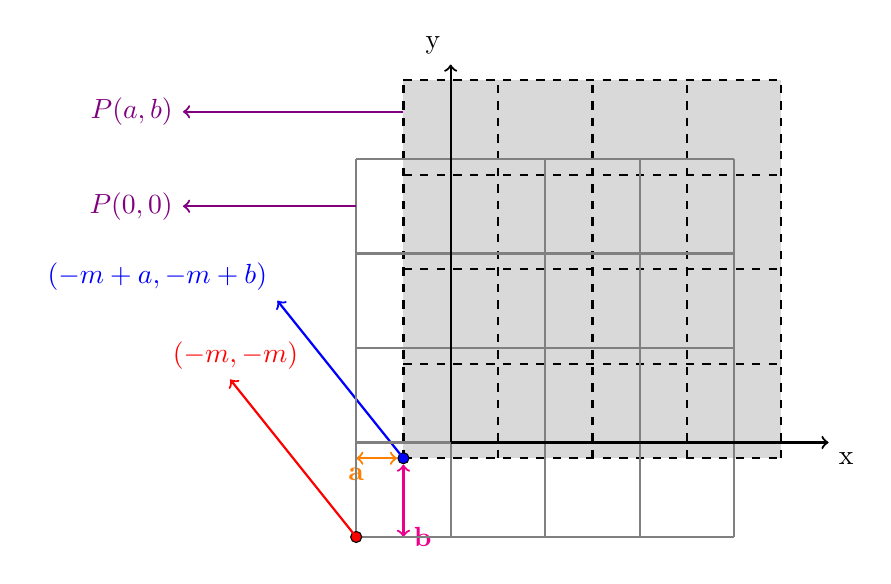
\begin{tikzpicture}[scale=0.4]

    \fill[gray!30] (0,0) rectangle (12,12);

   

    % Second Grid (dashed), positioned 2 units left and 3 units below
   
    \draw[step=3cm,black,dashed, thick] (0,0) grid (12,12);
    \filldraw[fill=blue] circle (5pt) ;
    \draw[orange, <->, thick] (-0.2, 0) -- (-1.5, 0) node[below] {\textbf{a}};
    \draw[magenta, <->, thick] (0, -0.2) -- (0, -2.5) node[right] {\textbf{b}};
    \draw[blue, ->, thick] (0, 0) -- (-4, 5) node[anchor=south east] {\textbf{ $(-m+a,-m+b)$}};

    
    

    \begin{scope}[xshift=-1.5cm, yshift=-2.5cm]
        \draw[step=3cm,gray, thick] (0,0) grid (12,12);
        \filldraw[fill=red] circle (5pt) ;
        \draw[red, ->, thick] (0, 0) -- (-4, 5) node[above] {\textbf{ $(-m,-m)$}};
        \draw[thick,->,black] (3,3) -- (15,3) node[anchor=north west] {x};
        \draw[thick,->,black] (3,3) -- (3,15) node[anchor=south east] {y};
    \end{scope}

    \draw[thick,->,violet] (0,11) -- (-7,11) node[left] {$P(a,b)$};
    \draw[thick,->,violet] (-1.5,8) -- (-7,8) node[left] {$P(0,0)$};

\end{tikzpicture}
\end{center}

%\draw[blue, ->, thick] (13.5, 13.5) -- (16, 15) node[right] {\textbf{\textit{\huge $\frac{1}{\sqrt{2}} \times \frac{1}{\sqrt{2}}$}}};

\end{frame}



\section{Theorem 4.4}

\begin{frame}

\begin{block}{Theorem 4.4}

    For any $\varepsilon > 0$, there is a $(1 + \varepsilon)$-approximation for the minimum dominating set problem in unit disk graphs that runs in time $n^{O(1/\varepsilon^2)}$.

\end{block}

\end{frame}

\begin{frame}{Theorem 4.4}

    \begin{center}
\begin{tikzpicture}[scale=1]

  

    % Whitebox System (3D effect)
   \node[draw, rectangle, minimum width=2cm, minimum height=1cm] (input) at (-3,0) {$UDG(V,E)$};

    % Whitebox System (3D effect)
    \node[draw, fill=gray!20, minimum width=2.5cm, minimum height=1.5cm] (whitebox) at (0.5, 0) {
        \begin{tikzpicture}[scale=0.75]
            \fill[gray!30] (0,0) rectangle (2.5, 1.5); % Front face
            \fill[gray!20] (0,0) -- (1,0.5) -- (1, 2) -- (0, 1.5) -- cycle; % Left face
            \fill[gray!15] (2.5,0) -- (3.5,0.5) -- (3.5, 2) -- (2.5, 1.5) -- cycle; % Right face
            \fill[gray!15] (1,2) -- (3.5, 2) -- (2.5,1.5)  -- (0, 1.5) -- cycle; % Upper face
            \draw (0,0) rectangle (2.5, 1.5); % Front edge
            \draw (0,0) -- (1,0.5) -- (1, 2) -- (0,1.5); % Left edges
            \draw (2.5,0) -- (3.5,0.5) -- (3.5, 2) -- (2.5,1.5); % Right edges
            \draw (1,0.5) -- (3.5,0.5);
            \draw (1,2) -- (3.5,2);
            
        \end{tikzpicture}
    };

    % Blackbox System (3D effect)
    \node[draw, fill=gray!20, text=white, minimum width=2.5cm, minimum height=1.5cm] (blackbox) at (6, 0) {
        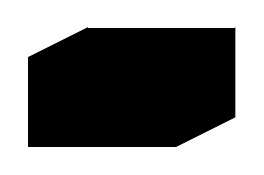
\begin{tikzpicture}[scale=0.75]
            \fill[gray!200] (0,0) rectangle (2.5, 1.5); % Front face
            \fill[gray!200] (0,0) -- (1,0.5) -- (1, 2) -- (0, 1.5) -- cycle; % Left face
            \fill[gray!200] (2.5,0) -- (3.5,0.5) -- (3.5, 2) -- (2.5, 1.5) -- cycle; % Right face
            \fill[gray!200] (1,2) -- (3.5, 2) -- (2.5,1.5)  -- (0, 1.5) -- cycle;
            \draw (0,0) rectangle (2.5, 1.5); % Front edge
            \draw (0,0) -- (1,0.5) -- (1, 2)-- (0,1.5); % Left edges
            \draw (2.5,0) -- (3.5,0.5) -- (3.5, 2)-- (2.5,1.5); % Right edges
            \draw (1,0.5) -- (3.5,0.5);
            \draw (1,2) -- (3.5,2);
        \end{tikzpicture}
    };

    % Output Node
    \node[draw, rectangle, minimum width=2cm, minimum height=1cm] (output_black) at (6, -3) {Result};

    % Draw arrows
    \draw[->] (input) -- (whitebox);
    \draw[->] (whitebox) -- (blackbox) node[midway, below]{diametre = 2};
    \draw[->] (whitebox) -- (blackbox) node[midway, above]{$UDG(V,E)$};
    \draw[->] (blackbox) -- (output_black);
    \node at (0.5,0) {$CDS-UDG$};
    \node at (6,0) {\textcolor{white}{$UDC_1$}};


\end{tikzpicture}
\end{center}

% The CDS-UDG implies that if u can dominate to a set of vertices V, it means that the vertices are UDC covered by a disk centered at u and diameter 2. Hence if G has k size Dominating set, then it means that the set of v vertices can be covered by k disc. Is my explanation for the reduction correct?
    
\end{frame}

\begin{frame}{Theorem 4.4 contd...}

    \begin{center}
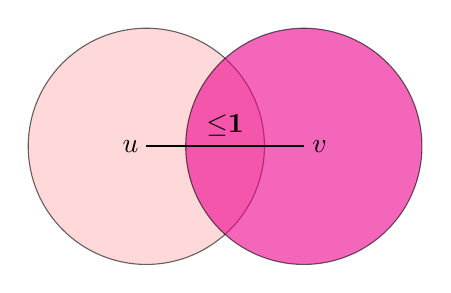
\begin{tikzpicture}

    % Draw the first circle (pink)
    \draw[fill=pink, opacity=0.6] (0,0) circle (1.5cm); 
    \node at (-0.2, 0) {\textbf{$u$}}; % Label the center as u
    
    % Draw the second circle (magenta) touching the first
    \draw[fill=magenta, opacity=0.6] (2,0) circle (1.5cm);
    \node at (2.2, 0) {\textbf{$v$}}; % Label the center as v
    
    % Draw the line between the centers and label it
    \draw[thick] (0,0) -- (2,0) node[midway, above] {\textbf{$\le$1}};
    
\end{tikzpicture}
\end{center}
    
\end{frame}

\begin{frame}{Theorem 4.4 contd...}

    


\begin{center}
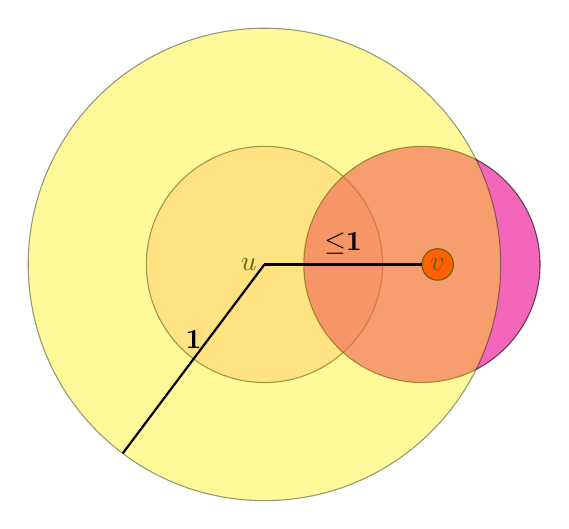
\begin{tikzpicture}

    % Draw the first circle (pink)
    \draw[fill=pink, opacity=0.6] (0,0) circle (1.5cm); 
    \node at (-0.2, 0) {\textbf{$u$}}; % Label the center as u
    
    % Draw the second circle (magenta) touching the first
    \draw[fill=magenta, opacity=0.6] (2,0) circle (1.5cm);
    \draw[fill=red, opacity=1] (2.2,0) circle (0.2cm);
    \node at (2.2, 0) {\textbf{$v$}}; % Label the center as v

    \draw[fill=yellow, opacity=0.4] (0,0) circle (3cm);

    
    
    % Draw the line between the centers and label it
    \draw[thick] (0,0) -- (2,0) node[midway, above] {\textbf{$\le$1}};
    \draw[thick] (0,0) -- (-1.8,-2.4) node[midway, above] {\textbf{1}};
    
    
\end{tikzpicture}
\end{center}
    
\end{frame}

\begin{frame}{Theorem 4.4 contd...}

    \begin{center}
\begin{tikzpicture}[scale=1]

  

    % Whitebox System (3D effect)
   \node[draw, rectangle, minimum width=2cm, minimum height=1cm] (input) at (-3,0) {$UDG(V,E)$};

    % Whitebox System (3D effect)
    \node[draw, fill=gray!20, minimum width=2.5cm, minimum height=1.5cm] (whitebox) at (0.5, 0) {
        \begin{tikzpicture}[scale=0.75]
            \fill[gray!30] (0,0) rectangle (2.5, 1.5); % Front face
            \fill[gray!20] (0,0) -- (1,0.5) -- (1, 2) -- (0, 1.5) -- cycle; % Left face
            \fill[gray!15] (2.5,0) -- (3.5,0.5) -- (3.5, 2) -- (2.5, 1.5) -- cycle; % Right face
            \fill[gray!15] (1,2) -- (3.5, 2) -- (2.5,1.5)  -- (0, 1.5) -- cycle; % Upper face
            \draw (0,0) rectangle (2.5, 1.5); % Front edge
            \draw (0,0) -- (1,0.5) -- (1, 2) -- (0,1.5); % Left edges
            \draw (2.5,0) -- (3.5,0.5) -- (3.5, 2) -- (2.5,1.5); % Right edges
            \draw (1,0.5) -- (3.5,0.5);
            \draw (1,2) -- (3.5,2);
            
        \end{tikzpicture}
    };

    % Blackbox System (3D effect)
    \node[draw, fill=gray!20, text=white, minimum width=2.5cm, minimum height=1.5cm] (blackbox) at (6, 0) {
        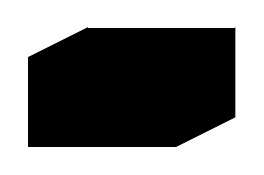
\begin{tikzpicture}[scale=0.75]
            \fill[gray!200] (0,0) rectangle (2.5, 1.5); % Front face
            \fill[gray!200] (0,0) -- (1,0.5) -- (1, 2) -- (0, 1.5) -- cycle; % Left face
            \fill[gray!200] (2.5,0) -- (3.5,0.5) -- (3.5, 2) -- (2.5, 1.5) -- cycle; % Right face
            \fill[gray!200] (1,2) -- (3.5, 2) -- (2.5,1.5)  -- (0, 1.5) -- cycle;
            \draw (0,0) rectangle (2.5, 1.5); % Front edge
            \draw (0,0) -- (1,0.5) -- (1, 2)-- (0,1.5); % Left edges
            \draw (2.5,0) -- (3.5,0.5) -- (3.5, 2)-- (2.5,1.5); % Right edges
            \draw (1,0.5) -- (3.5,0.5);
            \draw (1,2) -- (3.5,2);
        \end{tikzpicture}
    };

    % Output Node
    \node[draw, rectangle, minimum width=2cm, minimum height=1cm] (output_black) at (6, -3) {Result};

    % Draw arrows
    \draw[->] (input) -- (whitebox);
    \draw[->] (whitebox) -- (blackbox) node[midway, below]{diametre = 2};
    \draw[->] (whitebox) -- (blackbox) node[midway, above]{$UDG(V,E)$};
    \draw[->] (blackbox) -- (output_black);
    \node at (0.5,0) {$CDS-UDG$};
    \node at (6,0) {\textcolor{white}{$UDC_1$}};


\end{tikzpicture}
\end{center}

% The CDS-UDG implies that if u can dominate to a set of vertices V, it means that the vertices are UDC covered by a disk centered at u and diameter 2. Hence if G has k size Dominating set, then it means that the set of v vertices can be covered by k disc. Is my explanation for the reduction correct?
    
\end{frame}

\section{ A Lemma We need to know } 

\begin{frame}

    \begin{block}{A Lemma We need to know}

        If a Dominating set $D$ of some graph $G$ is not connected, then the number of its connected components can be reduced by adding at most two vertices to $D$

    \end{block}
    
\end{frame}

\begin{frame}{}


\begin{tikzpicture}
    % Shift the whole diagram down
    \node at (0,3) { % Place it 3 inches from the bottom
        \begin{tikzpicture}
            % Draw the two circles (without the radius being visible)
            \filldraw[fill=pink] (-3, 0) circle (1) node {D$_1$};
            \filldraw[fill=orange!50] (4, 0) circle (1) node {D$_2$};

            % Define points: v1 on the boundary of the pink circle, vm on the boundary of the orange circle
            \coordinate (v1) at (-2, 0);  % v1 on the rightmost point of the pink circle's boundary
            \coordinate (v2) at (-1, -0.5); % Intermediate points
            \coordinate (v3) at (0, 0.5);
            \coordinate (v4) at (1, -0.5);
            \coordinate (v5) at (2, 0.5);
            \coordinate (vm) at (3, 0);    % vm on the leftmost point of the orange circle's boundary

            % Draw the dotted zigzag edges
            \draw (v1) -- (v2);
            \draw (v2) -- (v3);
            \draw (v3) -- (v4);
            \draw (v4) -- (v5);
            \draw[dashed, thick] (v5) -- (vm);

            % Draw and label the points
            \filldraw[fill=black] (v1) circle (3pt) node[above] {v$_1$};
            \filldraw[fill=black] (v2) circle (3pt) node[below] {v$_2$};
            \filldraw[fill=black] (v3) circle (3pt) node[above] {v$_3$};
            \filldraw[fill=black] (v4) circle (3pt) node[below] {v$_4$};
            \filldraw[fill=black] (v5) circle (3pt) node[above] {v$_5$};
            \filldraw[fill=black] (vm) circle (3pt) node[below] {v$_m$};


            \node[draw, fill=blue!20, text width=10cm, rounded corners] at (0, -3) {
                $D_1$ and $D_2$ are the two connected components of the entire dominating set of vertices $D$ of some graph $G$ that are connected with the shortest possible path among connecting components $\{v_1, v_2, v_3, \dots, v_m\}$ where $v_1 \hspace{0.1em} \epsilon \hspace{0.1em} D_1$ and $v_m \hspace{0.1em} \epsilon \hspace{0.1em} D_2$.
            };
        
        \end{tikzpicture}
    };
\end{tikzpicture}



\end{frame}

\begin{frame}{A Lemma We need to know}




\begin{tikzpicture}
    % Draw the two circles (without radius visualization)
    \node at (0,3) {

        \begin{tikzpicture}
            \filldraw[fill=pink] (-3, 0) circle (1) node {D$_1$};
            \filldraw[fill=orange!50] (4, 0) circle (1) node {D$_2$};

            % Define points: v1 on the boundary of the pink circle, vm on the boundary of the orange circle
            \coordinate (v1) at (-2, 0);  % v1 on the rightmost point of the pink circle's boundary
            \coordinate (v2) at (-1, -0.5); % Intermediate points
            \coordinate (v3) at (0, 0.5);
            \coordinate (v4) at (1, -0.5);
            \coordinate (v5) at (2, 0.5);
            \coordinate (vm) at (3, 0);    % vm on the leftmost point of the orange circle's boundary

            % Draw the dotted zigzag edges
            \draw (v1) -- (v2);
            \draw [thick, blue](v2) -- (v3);
            \draw [thick, blue](v3) -- (v4);
            \draw [thick, blue](v4) -- (v5);
            \draw[dashed, thick, blue] (v5) -- (vm);

            % Draw and label the points
            \filldraw[fill=black] (v1) circle (3pt) node[above] {v$_1$};
            \filldraw[fill=black] (v2) circle (3pt) node[below] {v$_2$};
            \filldraw[fill=black] (v3) circle (3pt) node[above] {v$_3$};
            \filldraw[fill=black] (v4) circle (3pt) node[below] {v$_4$};
            \filldraw[fill=black] (v5) circle (3pt) node[above] {v$_5$};
            \filldraw[fill=black] (vm) circle (3pt) node[below] {v$_m$};

            % Draw the points: v2 to vm in blue
            \filldraw[fill=black] (v1) circle (3pt) node[above] {v$_1$};
            \filldraw[fill=blue] (v2) circle (3pt) node[below] {v$_2$};
            \filldraw[fill=blue] (v3) circle (3pt) node[above] {v$_3$};
            \filldraw[fill=blue] (v4) circle (3pt) node[below] {v$_4$};
            \filldraw[fill=blue] (v5) circle (3pt) node[above] {v$_5$};
            \filldraw[fill=blue] (vm) circle (3pt) node[below] {v$_m$};

             % Add the blue circle touching v2
            \filldraw[fill=blue, opacity = 0.4] (v2) ++(0, -1) circle (1) node {D$_3$}; % Circle below v2

            \node[draw, fill=blue!20, text width=10cm, rounded corners] at (0, -4) {
            Now $v_2$ cannot be a part of the Dominating set $D$ of the graph $G$ as this will give a shorter path $\{v_2, v_3, v_4, \dots, v_m\}$ contradicting to our assumption.
            };

        \end{tikzpicture}
    
    };

\end{tikzpicture}




\end{frame}

\begin{frame}{A Lemma We need to know}

\begin{tikzpicture}
    % Shift the whole diagram down
    \node at (0,3) { % Place it 3 inches from the bottom
        \begin{tikzpicture}
            % Draw the two circles (without the radius being visible)
            \filldraw[fill=pink] (-3, 0) circle (1) node {D$_1$};
            \filldraw[fill=orange!50] (4, 0) circle (1) node {D$_2$};

            % Define points: v1 on the boundary of the pink circle, vm on the boundary of the orange circle
            \coordinate (v1) at (-2, 0);  % v1 on the rightmost point of the pink circle's boundary
            \coordinate (v2) at (-1, -0.5); % Intermediate points
            \coordinate (v3) at (0, 0.5);
            \coordinate (v4) at (1, -0.5);
            \coordinate (v5) at (2, 0.5);
            \coordinate (vm) at (3, 0);    % vm on the leftmost point of the orange circle's boundary

            
            % Draw the dotted zigzag edges
            \draw (v1) -- (v2);
            \draw (v2) -- (v3);
            \draw (v3) -- (v4);
            \draw (v4) -- (v5);
            \draw[dashed, thick] (v5) -- (vm);

            % Draw and label the points
            \filldraw[fill=black] (v1) circle (3pt) node[above] {v$_1$};
            \filldraw[fill=black] (v2) circle (3pt) node[below] {v$_2$};
            \draw[thick, red] (v2) circle (10pt) ;
            \filldraw[fill=black] (v3) circle (3pt) node[above] {v$_3$};
            \filldraw[fill=black] (v4) circle (3pt) node[below] {v$_4$};
            \filldraw[fill=black] (v5) circle (3pt) node[above] {v$_5$};
            \filldraw[fill=black] (vm) circle (3pt) node[below] {v$_m$};
            


            \filldraw[fill=blue, opacity = 0.4] (v3) ++(0, 0.6) circle (0.6) node {D$_3$}; % Circle below v2

            

            \node[draw, fill=blue!20, text width=10cm, rounded corners] at (0, -4) {
            If $v_3 \hspace{0.1em} \epsilon \hspace{0.1em} D$, $v_2$ can be included in $D$ in order to reduce the number of connected components.
            };
        
        \end{tikzpicture}
    };
\end{tikzpicture}



\end{frame}

\begin{frame}{A Lemma We need to know}

\begin{tikzpicture}
    % Shift the whole diagram down
    \node at (0,3) { % Place it 3 inches from the bottom
        \begin{tikzpicture}
            % Draw the two circles (without the radius being visible)
            \filldraw[fill=pink] (-3, 0) circle (1) node {D$_1$};
            \filldraw[fill=orange!50] (4, 0) circle (1) node {D$_2$};

            % Define points: v1 on the boundary of the pink circle, vm on the boundary of the orange circle
            \coordinate (v1) at (-2, 0);  % v1 on the rightmost point of the pink circle's boundary
            \coordinate (v2) at (-1, -0.5); % Intermediate points
            \coordinate (v3) at (0, 0.5);
            \coordinate (v4) at (1, -0.5);
            \coordinate (v5) at (2, 0.5);
            \coordinate (vm) at (3, 0);    % vm on the leftmost point of the orange circle's boundary

            \filldraw[fill=yellow, opacity = 0.7] (v2)++(-1, 1) ellipse (3 and 2) node[above] {\textbf{D$_{1,3}$}};

            % Draw the dotted zigzag edges
            \draw (v1) -- (v2);
            \draw (v2) -- (v3);
            \draw (v3) -- (v4);
            \draw (v4) -- (v5);
            \draw[dashed, thick] (v5) -- (vm);

            % Draw and label the points
            \filldraw[fill=black] (v1) circle (3pt) node[above] {v$_1$};
            \filldraw[fill=black] (v2) circle (3pt) node[below] {v$_2$};
            \draw[thick, red] (v2) circle (10pt) ;
            \filldraw[fill=black] (v3) circle (3pt) node[above] {v$_3$};
            \filldraw[fill=black] (v4) circle (3pt) node[below] {v$_4$};
            \filldraw[fill=black] (v5) circle (3pt) node[above] {v$_5$};
            \filldraw[fill=black] (vm) circle (3pt) node[below] {v$_m$};
            


            \filldraw[fill=blue, opacity = 0.4] (v3) ++(0, 0.6) circle (0.6) node {D$_3$}; % Circle below v2

            

            \node[draw, fill=blue!20, text width=10cm, rounded corners] at (0, -3) {
            $D_1$ and $D_3$ are merged upon joining $v_2$ hence number of connected components reduced.
            };
        
        \end{tikzpicture}
    };
\end{tikzpicture}



\end{frame}

\begin{frame}{A Lemma We need to know}

\begin{tikzpicture}
    % Shift the whole diagram down
    \node at (0,3) { % Place it 3 inches from the bottom
        \begin{tikzpicture}
            % Draw the two circles (without the radius being visible)
            \filldraw[fill=pink] (-3, 0) circle (1) node {D$_1$};
            \filldraw[fill=orange!50] (4, 0) circle (1) node {D$_2$};

            % Define points: v1 on the boundary of the pink circle, vm on the boundary of the orange circle
            \coordinate (v1) at (-2, 0);  % v1 on the rightmost point of the pink circle's boundary
            \coordinate (v2) at (-1, -0.5); % Intermediate points
            \coordinate (v3) at (0, 0.5);
            \coordinate (v4) at (1, -0.5);
            \coordinate (v5) at (2, 0.5);
            \coordinate (vm) at (3, 0);    % vm on the leftmost point of the orange circle's boundary
            \coordinate (u) at (0, -1);

            

            % Draw the dotted zigzag edges
            \draw (v1) -- (v2);
            \draw [thick, blue](v2) -- (v3);
            \draw[thick, blue] (v3) -- (v4);
            \draw (v4) -- (v5);
            \draw[thick, blue] (v3) -- (u);
            \draw[dashed, thick] (v5) -- (vm);

            % Draw and label the points
            \filldraw[fill=black] (v1) circle (3pt) node[above] {v$_1$};
            \filldraw[fill=black] (v2) circle (3pt) node[below] {v$_2$};
            \draw[thick, red] (v2) circle (10pt) ;
            \filldraw[fill=black] (v3) circle (3pt) node[above] {v$_3$};
            \filldraw[fill=black] (v4) circle (3pt) node[below] {v$_4$};
            \draw[thick, red] (v4) circle (10pt) ;
            \filldraw[fill=black] (v5) circle (3pt) node[above] {v$_5$};
            \filldraw[fill=black] (vm) circle (3pt) node[below] {v$_m$};
            \filldraw[fill=black] (u) circle (3pt) node[below] {u};
            \draw[thick, red] (u) circle (10pt) ;
            


            \filldraw[fill=blue, opacity = 0.4] (u) ++(0, -1) circle (1) node {D$_3$}; % Circle below v2

            

            \node[draw, fill=blue!20, text width=10cm, rounded corners] at (0, -4) {
            If $v_3 \hspace{0.1em} \epsilon \hspace{-0.3em} | \hspace{0.1em} D$, then $v_3$ must be dominated by one of its neighbours $\{v_2, v_4, u\}$
            };
        
        \end{tikzpicture}
    };
\end{tikzpicture}



\end{frame}

\begin{frame}{A Lemma We need to know}

\begin{tikzpicture}
    % Shift the whole diagram down
    \node at (0,3) { % Place it 3 inches from the bottom
        \begin{tikzpicture}
            % Draw the two circles (without the radius being visible)
            \filldraw[fill=pink] (-3, 0) circle (1) node {D$_1$};
            \filldraw[fill=orange!50] (4, 0) circle (1) node {D$_2$};

            % Define points: v1 on the boundary of the pink circle, vm on the boundary of the orange circle
            \coordinate (v1) at (-2, 0);  % v1 on the rightmost point of the pink circle's boundary
            \coordinate (v2) at (-1, -0.5); % Intermediate points
            \coordinate (v3) at (0, 0.5);
            \coordinate (v4) at (1, -0.5);
            \coordinate (v5) at (2, 0.5);
            \coordinate (vm) at (3, 0);    % vm on the leftmost point of the orange circle's boundary
            \coordinate (u) at (0, -1);

            

            % Draw the dotted zigzag edges
            \draw (v1) -- (v2);
            \draw [thick, blue](v2) -- (v3);
            \draw[thick, blue] (v3) -- (v4);
            \draw (v4) -- (v5);
            \draw[thick, blue] (v3) -- (u);
            \draw[dashed, thick] (v5) -- (vm);

            % Draw and label the points
            \filldraw[fill=black] (v1) circle (3pt) node[above] {v$_1$};
            \filldraw[fill=black] (v2) circle (3pt) node[below] {v$_2$};
            \draw[thick, red] (v2) circle (10pt) ;
            \filldraw[fill=black] (v3) circle (3pt) node[above] {v$_3$};
            \filldraw[fill=black] (v4) circle (3pt) node[below] {v$_4$};
            \draw[thick, red] (v4) circle (10pt) ;
            \filldraw[fill=black] (v5) circle (3pt) node[above] {v$_5$};
            \filldraw[fill=black] (vm) circle (3pt) node[below] {v$_m$};
            \filldraw[fill=black] (u) circle (3pt) node[below] {u};
            \draw[thick, red] (u) circle (10pt) ;
            


            \filldraw[fill=blue, opacity = 0.4] (u) ++(0, -1) circle (1) node {D$_3$}; % Circle below v2

            

            \node[draw, fill=blue!20, text width=10cm, rounded corners] at (0, -4) {
            $\xrightarrow{}$ We already know $v_2 \hspace{0.1em} \epsilon \hspace{-0.3em} | \hspace{0.1em} D$
            
            $\xrightarrow{}$ If $v_4 \hspace{0.1em} \epsilon \hspace{0.1em} D$ or some $u \hspace{0.1em} \epsilon \hspace{0.1em} D_3$ ( $D_3 = \hspace{-1.2em} / D_1 $), then $v_2$ and $v_3$ are added to reduce a component
            };
        
        \end{tikzpicture}
    };
\end{tikzpicture}


\end{frame}

\begin{frame}{A Lemma We need to know}




\begin{tikzpicture}
    % Draw the two circles (without radius visualization)
    \node at (0,3) {

        \begin{tikzpicture}
            \filldraw[fill=pink] (-3, 0) circle (1) node {D$_1$};
            \filldraw[fill=orange!50] (4, 0) circle (1) node {D$_2$};

            % Define points: v1 on the boundary of the pink circle, vm on the boundary of the orange circle
            \coordinate (v1) at (-2, 0);  % v1 on the rightmost point of the pink circle's boundary
            \coordinate (v2) at (-1, -0.5); % Intermediate points
            \coordinate (v3) at (0, 0.5);
            \coordinate (v4) at (1, -0.5);
            \coordinate (v5) at (2, 0.5);
            \coordinate (vm) at (3, 0);    % vm on the leftmost point of the orange circle's boundary
            \coordinate (u) at (-3,1);

            % Draw the dotted zigzag edges
            \draw (v1) -- (v2);
            \draw [thick, blue](u) -- (v3);
            \draw (v2) -- (v3);
            \draw [thick, blue](v3) -- (v4);
            \draw [thick, blue](v4) -- (v5);
            \draw[dashed, thick, blue] (v5) -- (vm);

            % Draw and label the points
            \filldraw[fill=black] (v1) circle (3pt) node[above] {v$_1$};
            \filldraw[fill=black] (v2) circle (3pt) node[below] {v$_2$};
            \filldraw[fill=black] (v3) circle (3pt) node[above] {v$_3$};
            \filldraw[fill=black] (v4) circle (3pt) node[below] {v$_4$};
            \filldraw[fill=black] (v5) circle (3pt) node[above] {v$_5$};
            \filldraw[fill=black] (vm) circle (3pt) node[below] {v$_m$};
            \filldraw[fill=black] (u) circle (3pt) node[above] {u};

            % Draw the points: v2 to vm in blue
            \filldraw[fill=black] (v1) circle (3pt) node[above] {v$_1$};
            \filldraw[fill=black] (v2) circle (3pt) node[below] {v$_2$};
            \filldraw[fill=blue] (u) circle (3pt) node[above] {u};
            \filldraw[fill=blue] (v3) circle (3pt) node[above] {v$_3$};
            \filldraw[fill=blue] (v4) circle (3pt) node[below] {v$_4$};
            \filldraw[fill=blue] (v5) circle (3pt) node[above] {v$_5$};
            \filldraw[fill=blue] (vm) circle (3pt) node[below] {v$_m$};

        

            \node[draw, fill=blue!20, text width=10cm, rounded corners] at (0, -4) {
            Again $u \epsilon \hspace{-0.3em} / D_1 $ as this will give yet another shorter path $\{u, v_3, v_4, \dots, v_m\}$ contradicting to our assumption.
            };

        \end{tikzpicture}
    
    };

\end{tikzpicture}




\end{frame}

\section{Theorem 4.5}

\begin{frame}



\begin{block}{Theorem 4.5}

    There is a polynomial-time 4-approximation for CDS-UDG.

\end{block}

\end{frame}

\begin{frame}{Theorem 4.5 contd...}

\begin{enumerate}

    \item Suppose the approximated Dominating set of a Unit Disk Graph $G(V,E)$ , $D \subseteq V$ is a (4/3)-approximation for the minimum connected Dominating set $D^*$


    $ |D| \le 4|D^*|/3$

    \item Our claim is that $D$ is not connected

    \item We have already proved that, If a Dominating set $D$ of some graph $G$ is not connected, then the number of its connected components can be reduced by adding at most two vertices to $D$

    \item Hence, as per our claim, we need to add at most $2(c -1)$ vertices to $D$ to get a connected dominating set, where $c$ is the number of connected components in $D$.
    
\end{enumerate}




\end{frame}

\begin{frame}{Theorem 4.5 contd...}

\begin{exampleblock}{Calculation for 4-approximation}

    Clearly, 
    $c-1 < c \le |D|$

    \vspace{5mm}
    
    $\xrightarrow{} 2(c-1) < 2|D|$

    \vspace{5mm}

    $\xrightarrow{} |D| + 2(c-1) < 3|D|$

    \vspace{5mm}

    $\xrightarrow{} |C| < 3|D|$

    \vspace{5mm}

    $\xrightarrow{} |C| < 3 ( 4|D^*|/3 )$

    \vspace{5mm}

    $\xrightarrow{} |C| < 4|D^*|$

\end{exampleblock}
    
\end{frame}

\section{We need to know more}

\begin{frame}{We need to know more}

\begin{center}
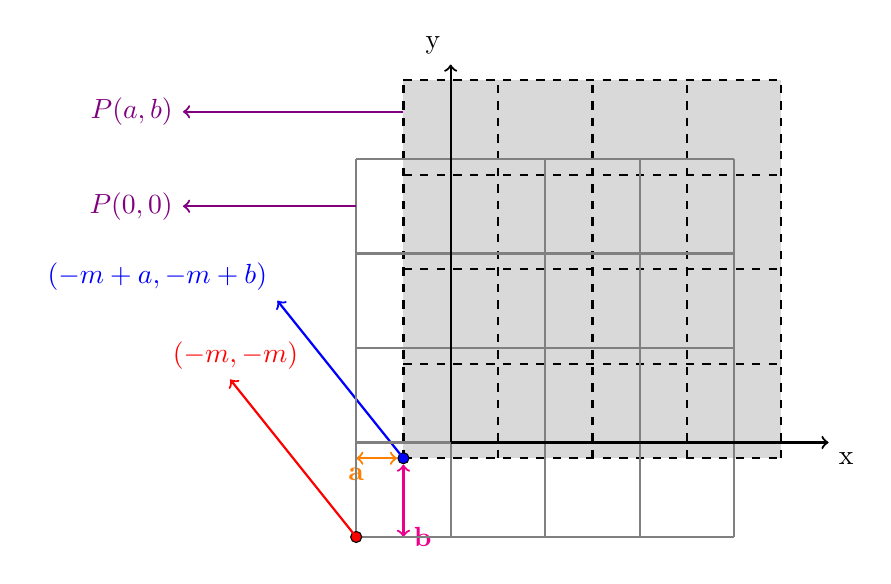
\begin{tikzpicture}[scale=0.4]

    \fill[gray!30] (0,0) rectangle (12,12);

   

    % Second Grid (dashed), positioned 2 units left and 3 units below
   
    \draw[step=3cm,black,dashed, thick] (0,0) grid (12,12);
    \filldraw[fill=blue] circle (5pt) ;
    \draw[orange, <->, thick] (-0.2, 0) -- (-1.5, 0) node[below] {\textbf{a}};
    \draw[magenta, <->, thick] (0, -0.2) -- (0, -2.5) node[right] {\textbf{b}};
    \draw[blue, ->, thick] (0, 0) -- (-4, 5) node[anchor=south east] {\textbf{ $(-m+a,-m+b)$}};

    
    

    \begin{scope}[xshift=-1.5cm, yshift=-2.5cm]
        \draw[step=3cm,gray, thick] (0,0) grid (12,12);
        \filldraw[fill=red] circle (5pt) ;
        \draw[red, ->, thick] (0, 0) -- (-4, 5) node[above] {\textbf{ $(-m,-m)$}};
        \draw[thick,->,black] (3,3) -- (15,3) node[anchor=north west] {x};
        \draw[thick,->,black] (3,3) -- (3,15) node[anchor=south east] {y};
    \end{scope}

    \draw[thick,->,violet] (0,11) -- (-7,11) node[left] {$P(a,b)$};
    \draw[thick,->,violet] (-1.5,8) -- (-7,8) node[left] {$P(0,0)$};

\end{tikzpicture}
\end{center}

%\draw[blue, ->, thick] (13.5, 13.5) -- (16, 15) node[right] {\textbf{\textit{\huge $\frac{1}{\sqrt{2}} \times \frac{1}{\sqrt{2}}$}}};

\end{frame}

\begin{frame}{Why Partition shifting?}

\begin{center}
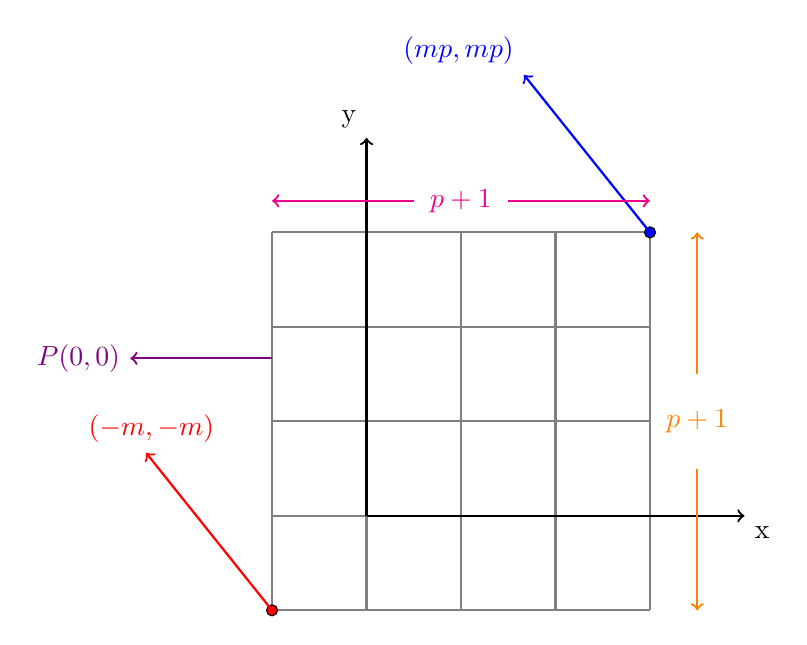
\begin{tikzpicture}[scale=0.4]

    %\fill[gray!30] (0,0) rectangle (12,12);

   

    % Second Grid (dashed), positioned 2 units left and 3 units below
   
    % \draw[step=3cm,black,dashed, thick] (0,0) grid (12,12);
    % \filldraw[fill=blue] circle (5pt) ;
    % \draw[orange, <->, thick] (-0.2, 0) -- (-1.5, 0) node[below] {\textbf{a}};
    % \draw[magenta, <->, thick] (0, -0.2) -- (0, -2.5) node[right] {\textbf{b}};
    % \draw[blue, ->, thick] (0, 0) -- (-4, 5) node[anchor=south east] {\textbf{ $(-m+a,-m+b)$}};

    
    

    %\begin{scope}[xshift=-1.5cm, yshift=-2.5cm]
        \draw[step=3cm,gray, thick] (0,0) grid (12,12);
        \filldraw[fill=red] circle (5pt) ;
        \filldraw[fill=blue](12,12) circle (5pt) ;
        \draw[red, ->, thick] (0, 0) -- (-4, 5) node[above] {\textbf{ $(-m,-m)$}};
        \draw[thick,->,black] (3,3) -- (15,3) node[anchor=north west] {x};
        \draw[thick,->,black] (3,3) -- (3,15) node[anchor=south east] {y};

        \draw[blue, ->, thick] (12, 12) -- (8, 17) node[anchor=south east] {\textbf{ $(mp,mp)$}};
        
    %\end{scope}

    %\draw[thick,->,violet] (0,11) -- (-7,11) node[left] {$P(a,b)$};
    \draw[thick,->,violet] (0,8) -- (-4.5,8) node[left] {$P(0,0)$};
    \draw[thick,->,magenta] (4.5,13) -- (0,13);
    \node[magenta] at (6,13) {$p+1$};
    \draw[thick,->,magenta] (7.5,13) -- (12,13);

    \draw[thick,->,orange] (13.5,4.5) -- (13.5,0);
    \node[orange] at (13.5,6) {$p+1$};
    \draw[thick,->,orange] (13.5, 7.5) -- (13.5,12);

    

\end{tikzpicture}
\end{center}

\end{frame}

\begin{frame}{Why Partition shifting?}





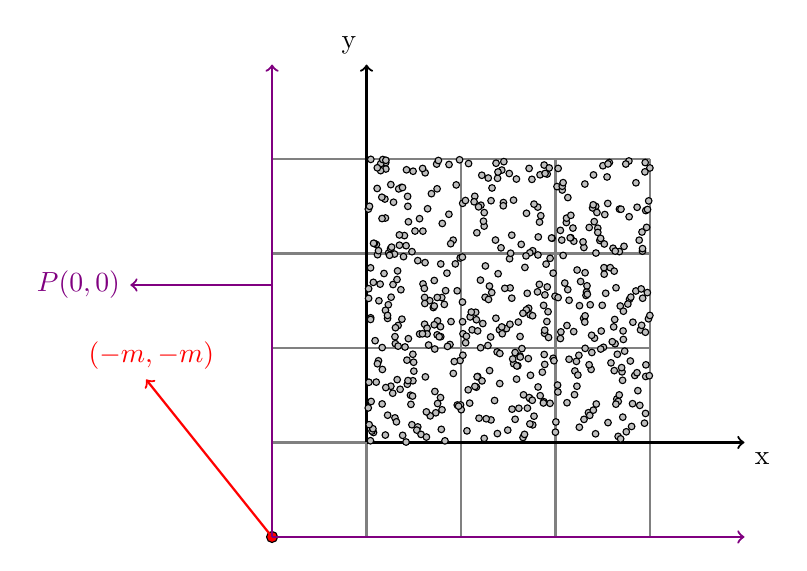
\begin{tikzpicture}[scale=0.4]

    % Draw the grid
    \draw[step=3cm,gray, thick] (0,0) grid (12,12);
    \filldraw[fill=red] circle (5pt) ;
        
    \draw[red, ->, thick] (0, 0) -- (-4, 5) node[above] {\textbf{ $(-m,-m)$}};
    \draw[thick,->,black] (3,3) -- (15,3) node[anchor=north west] {x};
    \draw[thick,->,black] (3,3) -- (3,15) node[anchor=south east] {y};

    \draw[thick,->,violet] (0,0) -- (15,0) ;
    \draw[thick,->,violet] (0,0) -- (0,15) ;

    \draw[thick,->,violet] (0,8) -- (-4.5,8) node[left] {$P(0,0)$};

    % Seed for randomness
    \pgfmathsetseed{42}  % Set seed for reproducibility

    % Generate 10 random points within the grid
    \foreach \i in {1,...,500} {
        \pgfmathsetmacro{\x}{3 + rnd*9}
        \pgfmathsetmacro{\y}{3 + rnd*9}
        \filldraw[fill=gray!50] (\x,\y) circle (3pt); % Draw a red point at random (x,y)
    }

\end{tikzpicture}


\end{frame}

\begin{frame}{Why Partition shifting?}

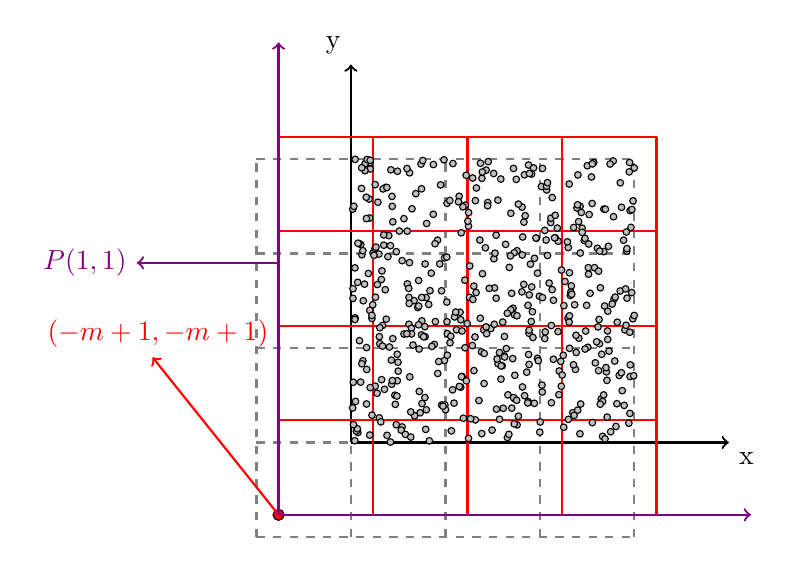
\begin{tikzpicture}[scale=0.4]

    % Draw the grid
    \draw[step=3cm,dashed, gray, thick] (0,0) grid (12,12);

    \draw[thick,->,black] (3,3) -- (15,3) node[anchor=north west] {x};
    \draw[thick,->,black] (3,3) -- (3,15) node[anchor=south east] {y};

    \begin{scope}[xshift = 20, yshift = 20]
    
    \filldraw[fill=red] circle (5pt) ;
        
    \draw[red, ->, thick] (0, 0) -- (-4, 5) node[above] {\textbf{ $(-m+1,-m+1)$}};

    \draw[step=3cm, red, thick] (0,0) grid (12,12);
    

    \draw[thick,->,violet] (0,0) -- (15,00) ;
    \draw[thick,->,violet] (0,0) -- (0,15) ;

    \draw[thick,->,violet] (0,8) -- (-4.5,8) node[left] {$P(1,1)$};

    \end{scope}

    % Seed for randomness
    \pgfmathsetseed{42}  % Set seed for reproducibility

    % Generate 10 random points within the grid
    \foreach \i in {1,...,500} {
        \pgfmathsetmacro{\x}{3 + rnd*9}
        \pgfmathsetmacro{\y}{3 + rnd*9}

        % \ifdim \x pt > 3pt \ifdim \x pt < 6pt \ifdim \y pt > 3pt \ifdim \y pt < 6pt
        %     \filldraw[fill=red] (\x,\y) circle (3pt); % Draw red point
        % \else
            \filldraw[fill=gray!50] (\x,\y) circle (3pt); % Draw gray point
        % \fi\fi\fi\else
        %     \filldraw[fill=gray!50] (\x,\y) circle (3pt); % Draw gray point
        % \fi
    }

\end{tikzpicture}

\end{frame}



\begin{frame}{Why Partition shifting?}

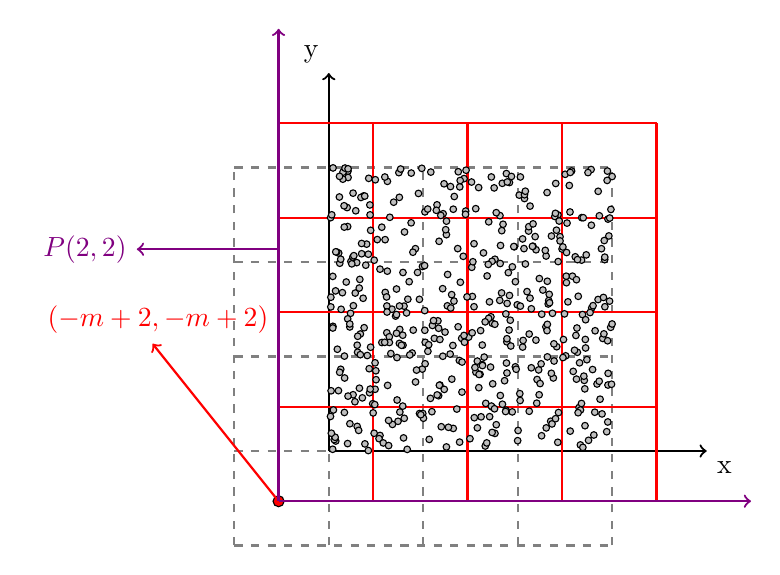
\begin{tikzpicture}[scale=0.4]

    % Draw the grid
    \draw[step=3cm,dashed, gray, thick] (0,0) grid (12,12);

    \draw[thick,->,black] (3,3) -- (15,3) node[anchor=north west] {x};
    \draw[thick,->,black] (3,3) -- (3,15) node[anchor=south east] {y};

    \begin{scope}[xshift = 40, yshift = 40]
    
    \filldraw[fill=red] circle (5pt) ;
        
    \draw[red, ->, thick] (0, 0) -- (-4, 5) node[above] {\textbf{ $(-m+2,-m+2)$}};

    \draw[step=3cm, red, thick] (0,0) grid (12,12);
    

    \draw[thick,->,violet] (0,0) -- (15,00) ;
    \draw[thick,->,violet] (0,0) -- (0,15) ;

    \draw[thick,->,violet] (0,8) -- (-4.5,8) node[left] {$P(2,2)$};

    \end{scope}

    % Seed for randomness
    \pgfmathsetseed{42}  % Set seed for reproducibility

    % Generate 10 random points within the grid
    \foreach \i in {1,...,500} {
        \pgfmathsetmacro{\x}{3 + rnd*9}
        \pgfmathsetmacro{\y}{3 + rnd*9}

        % \ifdim \x pt > 3pt \ifdim \x pt < 6pt \ifdim \y pt > 3pt \ifdim \y pt < 6pt
        %     \filldraw[fill=red] (\x,\y) circle (3pt); % Draw red point
        % \else
            \filldraw[fill=gray!50] (\x,\y) circle (3pt); % Draw gray point
        % \fi\fi\fi\else
        %     \filldraw[fill=gray!50] (\x,\y) circle (3pt); % Draw gray point
        % \fi
    }

\end{tikzpicture}

\end{frame}

\begin{frame}{Why Partition shifting?}

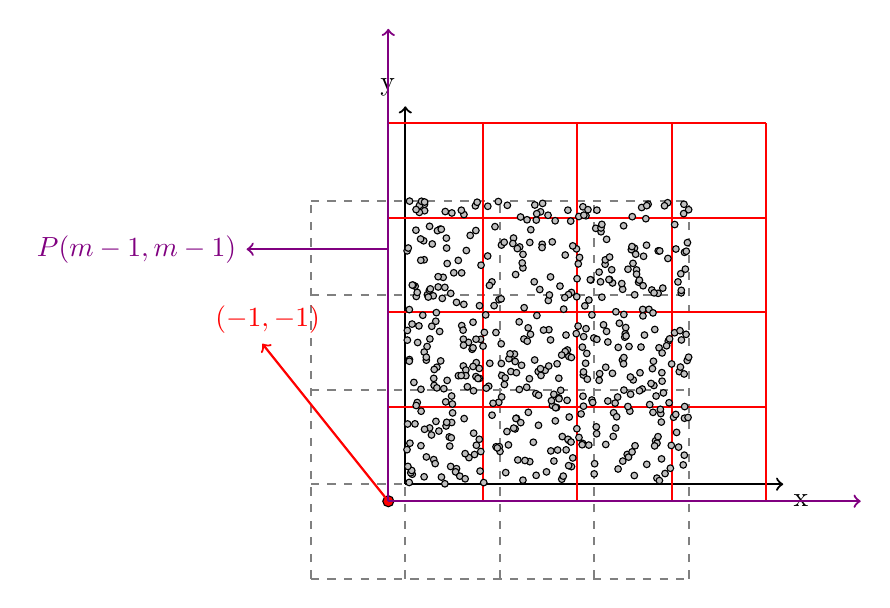
\begin{tikzpicture}[scale=0.4]

    % Draw the grid
    \draw[step=3cm,dashed, gray, thick] (0,0) grid (12,12);

    \draw[thick,->,black] (3,3) -- (15,3) node[anchor=north west] {x};
    \draw[thick,->,black] (3,3) -- (3,15) node[anchor=south east] {y};

    \begin{scope}[xshift = 70, yshift = 70]
    
    \filldraw[fill=red] circle (5pt) ;
        
    \draw[red, ->, thick] (0, 0) -- (-4, 5) node[above] {\textbf{ $(-1,-1)$}};

    \draw[step=3cm, red, thick] (0,0) grid (12,12);
    

    \draw[thick,->,violet] (0,0) -- (15,00) ;
    \draw[thick,->,violet] (0,0) -- (0,15) ;

    \draw[thick,->,violet] (0,8) -- (-4.5,8) node[left] {$P(m-1,m-1)$};

    \end{scope}

    % Seed for randomness
    \pgfmathsetseed{42}  % Set seed for reproducibility

    % Generate 10 random points within the grid
    \foreach \i in {1,...,500} {
        \pgfmathsetmacro{\x}{3 + rnd*9}
        \pgfmathsetmacro{\y}{3 + rnd*9}

        % \ifdim \x pt > 3pt \ifdim \x pt < 6pt \ifdim \y pt > 3pt \ifdim \y pt < 6pt
        %     \filldraw[fill=red] (\x,\y) circle (3pt); % Draw red point
        % \else
            \filldraw[fill=gray!50] (\x,\y) circle (3pt); % Draw gray point
        % \fi\fi\fi\else
        %     \filldraw[fill=gray!50] (\x,\y) circle (3pt); % Draw gray point
        % \fi
    }

\end{tikzpicture}

\end{frame}

\begin{frame}{Central Area and Boundary Area}

\begin{center}
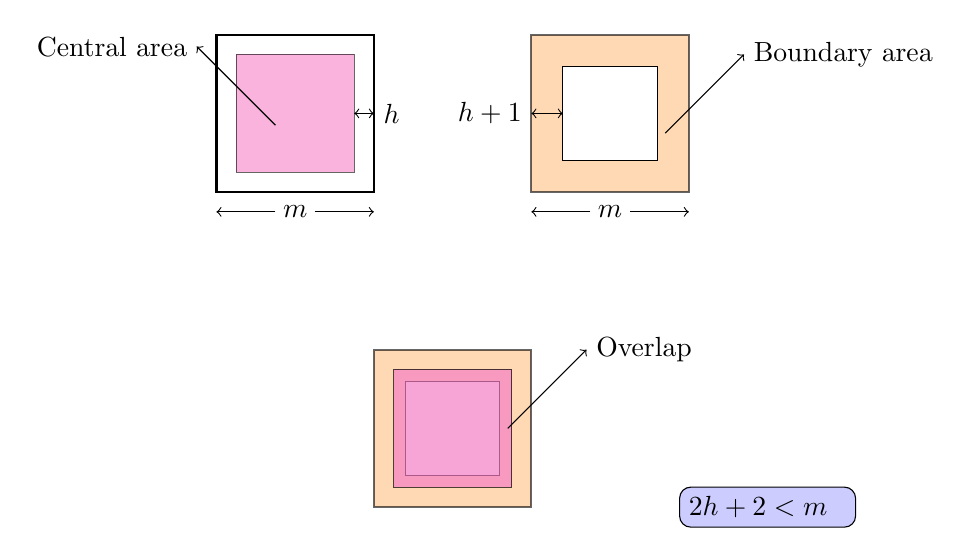
\begin{tikzpicture}

    % First square: Central area highlighted
    \draw[thick] (0, 2) rectangle ++(2, 2);
    \draw[fill=magenta!50, opacity = 0.6] (0.25, 2.25) rectangle ++(1.5, 1.5);
    \draw[->] (0.75, 2.85) -- ++(-1, 1) node[left] {Central area};
    \draw[->] (0.75, 1.75) -- (0, 1.75) ;
    \draw[->] (1.25, 1.75) -- (2, 1.75) ;
    \draw[<->] (1.75, 3) -- ++(0.25, 0) node[right] {$h$};
    \node at (1,1.75) {$m$};

    % Second square: Boundary area highlighted
    \draw[thick,fill=orange!50, opacity = 0.6] (4, 2) rectangle ++(2, 2);
    \draw[fill=white] (4.4, 2.4) rectangle ++(1.2, 1.2);
    \draw[->] (5.7, 2.75) -- ++(1, 1) node[right] {Boundary area};
    \draw[->] (4.75, 1.75) -- (4, 1.75) ;
    \draw[->] (5.25, 1.75) -- (6, 1.75) ;
    \draw[<->] (4.4, 3) -- ++(-0.4, 0) node[left] {$h +1$};
    \node at (5,1.75) {$m$};

    % Third square: Both areas highlighted
    \draw[thick, fill=orange!50, opacity = 0.6] (2, -2) rectangle ++(2, 2);
    \draw[fill=white] (2.4, -1.6) rectangle ++(1.2, 1.2);
    \draw[fill=magenta!50, opacity=0.7] (2.25, -1.75) rectangle ++(1.5, 1.5);
    \draw[->] (3.7, -1) -- ++(1, 1) node[right] {Overlap};

    \node[draw, fill=blue!20, text width=2cm, rounded corners] at (7, -2) {
           $2h + 2 < m$
            };
    

\end{tikzpicture}
\end{center}

\end{frame}

\begin{frame}{Central Area and Boundary Area}

\begin{center}
    

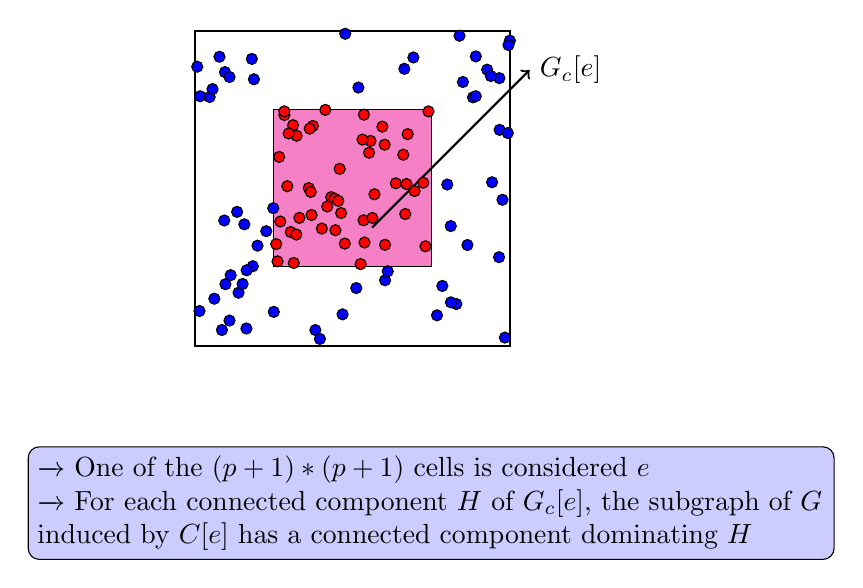
\begin{tikzpicture}

    % Square in the middle
    \draw[thick] (2, 2) rectangle ++(4, 4);
    \draw[fill=magenta!50] (3, 3) rectangle ++(2, 2);

    % Label for the central area
    \draw[->, thick] (4.25, 3.5) -- ++(2, 2) node[right] {$G_c[e]$};

    \pgfmathsetseed{42}

    % Random red points inside the central area
    \foreach \i in {1,...,50} {
        \pgfmathsetmacro{\x}{3 + rnd*2}
        \pgfmathsetmacro{\y}{3 + rnd*2}
        \filldraw[fill=red] (\x,\y)  circle (2pt);
        % (3 + rand*2, 3 + rand*2)
    }

    % Random blue points outside the central area but inside the square
    \foreach \i in {1,...,15} {
        \pgfmathsetmacro{\x}{2 + rnd}
        \pgfmathsetmacro{\y}{2 + rnd*4}
        \filldraw[fill=blue] (\x,\y)  circle (2pt);
    }

    \foreach \i in {1,...,15} {
        \pgfmathsetmacro{\x}{2 + rnd*4}
        \pgfmathsetmacro{\y}{2 + rnd}
        \filldraw[fill=blue] (\x,\y)  circle (2pt);
    }

    \foreach \i in {1,...,15} {
        \pgfmathsetmacro{\x}{5 + rnd}
        \pgfmathsetmacro{\y}{2 + rnd*4}
        \filldraw[fill=blue] (\x,\y)  circle (2pt);
    }

    \foreach \i in {1,...,15} {
        \pgfmathsetmacro{\x}{2 + rnd*4}
        \pgfmathsetmacro{\y}{5 + rnd}
        \filldraw[fill=blue] (\x,\y)  circle (2pt);
    }

    \node[draw, fill=blue!20, text width=10cm, rounded corners] at (5, 0) {
            $ \xrightarrow{} $ One of the $(p+1)*(p+1)$ cells is considered $e$
            
            $ \xrightarrow{} $ For each connected component $H$ of $G_c[e]$, the subgraph of $G$ induced by $C[e]$ has a connected component dominating $H$
            };

\end{tikzpicture}

\end{center}

\end{frame}

\section{Theorem 4.6}

\begin{frame}{}

\begin{block}{Theorem 4.6}

    For each cell $e$ in a partition $P(a, a)$, the set $C[e]$ can be computed in time $n _e ^ {O(m^2)}$  , where $n_e$ is the number of vertices in $e$

\end{block}

\end{frame}

\begin{frame}{Theorem 4.6}

    \begin{enumerate}

    \item We have already known that that each cell can be covered with $ 2m^2 $ unit disks without considering boundaries, hence there are at most $ 2m^2 $ dominating vertices in $C[e]$

    \item We have already proved that, If a Dominating set $D$ of some graph $G$ is not connected, then the number of its connected components can be reduced by adding at most two vertices to $D$, hence for making the set connected we add at most $ 2 * 2m^2 = 4m^2 $ more vertices to $C[e]$

    \item Hence, as per our claim, there at most $ 6m^2 $ vertices in $C[e]$ to get a connected dominating set, which are selected from $n_e$ vertices in cell $e$

    
\end{enumerate}

\end{frame}

\begin{frame}{Theorem 4.6 contd...}

    
    \begin{exampleblock}{Calculation for $C[e]$}

    At most $ 6m^2 $ vertices are exhaustively selected from $n_e$ vertices.

    \vspace{5mm}
    
    $ \xrightarrow{} \binom{n_e}{1} + \binom{n_e}{2} + \binom{n_e}{3} + ... + \binom{n_e}{6m^2} $

    \vspace{5mm}

    $\xrightarrow{} \displaystyle \sum_{k=1}^{6m^2} \binom{n_e}{k}$

    \vspace{5mm}

    $\xrightarrow{} n _e ^ {O(m^2)}$

    \vspace{5mm}

    Whether $ C[e] $ dominates each connected dominating set $H$ in subgraph $G_c[e]$ can be determine in linear time. So $C[e]$ is calculated in time $n _e ^ {O(m^2)}$

    \end{exampleblock}


\end{frame}

\section{PTAS for CDS-UDG}

\begin{frame}{PTAS for CDS-UDG}

% \renewcommand{\thealgorithm}{4.\arabic{algorithm}}


% \setcounter{algorithm}{0}

\renewcommand{\thealgorithm}{4.B}

\begin{algorithm}[H]

\caption{$\textbf{4.B}$ PTAS for CDS-UDG}
\textbf{Input:} A unit disk graph $G = (V, E)$, with all vertices lying in square $Q$.\\
\textbf{Output:} An approximate connected dominating set $A_{a^*}$.
\small
\begin{algorithmic}[1]
    \State Let $h \gets 3$ and $m \gets \lceil 160/\epsilon \rceil$.
    \State Let $D \subseteq V$ be a 4-approximation to the minimum connected dominating set for $G$ (obtained by the algorithm of Corollary 4.5).
    \For {$a \gets 0$ to $m - 1$}
        \State Let $D_a \gets \{v \in D \mid v \text{ lies in the boundary area of } P(a, a)\}$.
        \For {each cell $e$ of $P(a, a)$}
            \State Compute set $C[e]$ (by exhaustive search of Lemma 4.6).
        \EndFor
        \State Let $A_a \gets D_a \cup \left( \bigcup\limits_{e \in P(a,a)} C[e] \right)$.
    \EndFor
    \State Let $a^* \gets \arg\min\limits_{0 \leq a < m} |A_a|$.
    \State \textbf{Return} $A_{a^*}$.
\end{algorithmic}
\end{algorithm}



\end{frame}

\section{And we need to know again}

\begin{frame}{And we need to know again}

\begin{center}
    

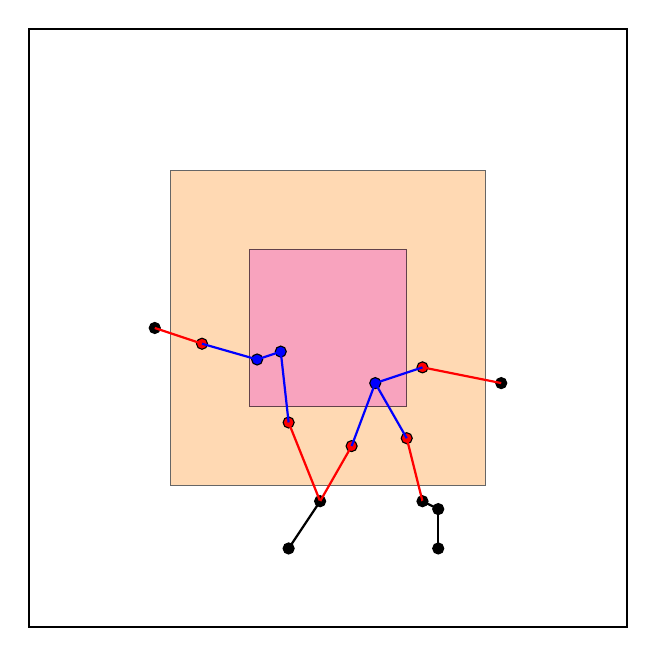
\begin{tikzpicture}

    % Square in the middle
    \draw[thick] (1.2, 1.2) rectangle ++(7.6, 7.6);
    \draw[fill=orange!50, opacity = 0.6] (3, 3) rectangle ++(4, 4);
    \draw[fill=magenta!50, opacity = 0.6] (4, 4) rectangle ++(2, 2);

    \coordinate (v1) at (2.8, 5);

    \filldraw[fill=black] (v1) circle (2pt);

    \coordinate (v6) at (4.9, 2.8);

    \filldraw[fill=black] (v6) circle (2pt);

    \coordinate (v72) at (4.5, 2.2);

    \filldraw[fill=black] (v72) circle (2pt);

    \coordinate (v9b) at (6.2, 2.8);

    \filldraw[fill=black] (v9b) circle (2pt);

    \coordinate (v9c) at (6.4, 2.7);

    \filldraw[fill=black] (v9c) circle (2pt);

    \coordinate (v9d) at (6.4, 2.2);

    \filldraw[fill=black] (v9d) circle (2pt);

    \coordinate (v92) at (7.2, 4.3);

    \filldraw[fill=black] (v92) circle (2pt);


    

    

    \coordinate (v2) at (3.4, 4.8);

    \filldraw[fill=red] (v2) circle (2pt);

    \coordinate (v5) at (4.5, 3.8);

    \filldraw[fill=red] (v5) circle (2pt);

    \coordinate (v71) at (5.3, 3.5);

    \filldraw[fill=red] (v71) circle (2pt);

    \coordinate (v9a) at (6, 3.6);

    \filldraw[fill=red] (v9a) circle (2pt);

    \coordinate (v91) at (6.2, 4.5);

    \filldraw[fill=red] (v91) circle (2pt);

    

    \coordinate (v3) at (4.1, 4.6);

    \filldraw[fill=blue] (v3) circle (2pt);

    \coordinate (v4) at (4.4, 4.7);

    \filldraw[fill=blue] (v4) circle (2pt);

    \coordinate (v8) at (5.6, 4.3);

    \filldraw[fill=blue] (v8) circle (2pt);

   



    \draw [thick, red](v1) -- (v2);
    \draw [thick, red](v5) -- (v6);
    \draw [thick, red](v6) -- (v71);
    \draw [thick, red](v91) -- (v92);
    \draw [thick, red](v9a) -- (v9b);


    \draw [thick, blue](v2) -- (v3);
    \draw [thick, blue](v4) -- (v5);
    \draw [thick, blue](v71) -- (v8);
    \draw [thick, blue](v8) -- (v9a);
    \draw [thick, blue](v8) -- (v91);
    


    \draw [thick, black](v6) -- (v72);
    \draw [thick, black](v9b) -- (v9c);
    \draw [thick, black](v9c) -- (v9d);


    \draw [thick, blue](v3) -- (v4);


    

\end{tikzpicture}

\end{center}



\end{frame}

\begin{frame}{How do we achieve $D_a$ ?}

\begin{center}
    

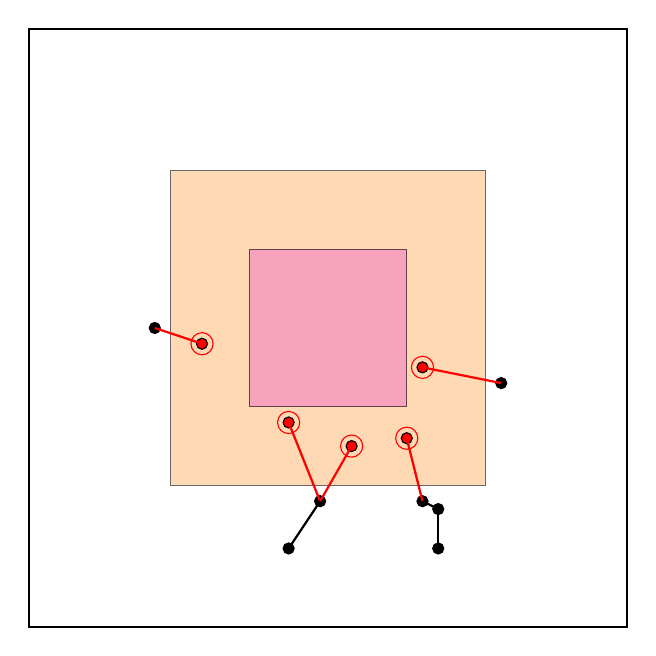
\begin{tikzpicture}

    % Square in the middle
    \draw[thick] (1.2, 1.2) rectangle ++(7.6, 7.6);
    \draw[fill=orange!50, opacity = 0.6] (3, 3) rectangle ++(4, 4);
    \draw[fill=magenta!50, opacity = 0.6] (4, 4) rectangle ++(2, 2);

    \coordinate (v1) at (2.8, 5);

    \filldraw[fill=black] (v1) circle (2pt);

    \coordinate (v6) at (4.9, 2.8);

    \filldraw[fill=black] (v6) circle (2pt);

    \coordinate (v72) at (4.5, 2.2);

    \filldraw[fill=black] (v72) circle (2pt);

    \coordinate (v9b) at (6.2, 2.8);

    \filldraw[fill=black] (v9b) circle (2pt);

    \coordinate (v9c) at (6.4, 2.7);

    \filldraw[fill=black] (v9c) circle (2pt);

    \coordinate (v9d) at (6.4, 2.2);

    \filldraw[fill=black] (v9d) circle (2pt);

    \coordinate (v92) at (7.2, 4.3);

    \filldraw[fill=black] (v92) circle (2pt);


    

    

    \coordinate (v2) at (3.4, 4.8);

    \filldraw[fill=red] (v2) circle (2pt);

    \draw[red] (v2) circle (4pt);

    \coordinate (v5) at (4.5, 3.8);

    \filldraw[fill=red] (v5) circle (2pt);

    \draw[red] (v5) circle (4pt);

    \coordinate (v71) at (5.3, 3.5);

    \filldraw[fill=red] (v71) circle (2pt);

    \draw[red] (v71) circle (4pt);

    \coordinate (v9a) at (6, 3.6);

    \filldraw[fill=red] (v9a) circle (2pt);

    \draw[red] (v9a) circle (4pt);

    \coordinate (v91) at (6.2, 4.5);

    \filldraw[fill=red] (v91) circle (2pt);

    \draw[red] (v91) circle (4pt);

    

    



    \draw [thick, red](v1) -- (v2);
    \draw [thick, red](v5) -- (v6);
    \draw [thick, red](v6) -- (v71);
    \draw [thick, red](v91) -- (v92);
    \draw [thick, red](v9a) -- (v9b);


    


    \draw [thick, black](v6) -- (v72);
    \draw [thick, black](v9b) -- (v9c);
    \draw [thick, black](v9c) -- (v9d);


   

    

\end{tikzpicture}

\end{center}



\end{frame}

\begin{frame}{How do we achieve $G_c[e]$ ?}

\begin{center}
    

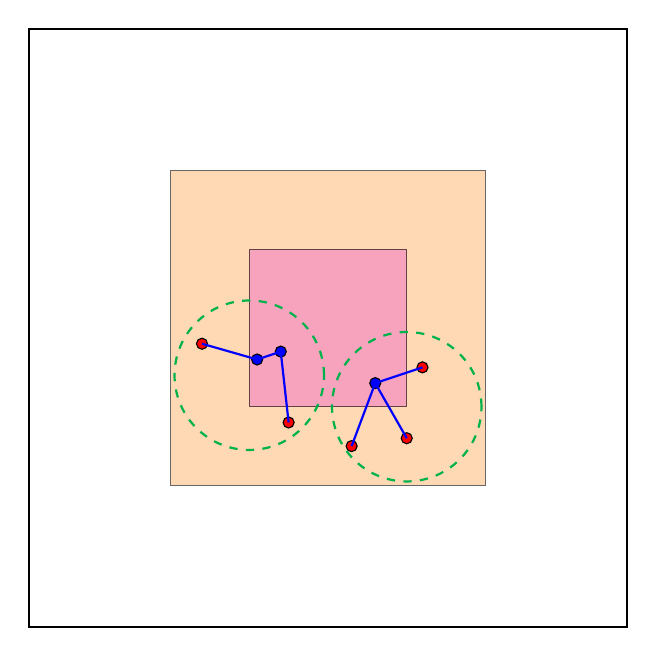
\begin{tikzpicture}

    % Square in the middle
    \draw[thick] (1.2, 1.2) rectangle ++(7.6, 7.6);
    \draw[fill=orange!50, opacity = 0.6] (3, 3) rectangle ++(4, 4);
    \draw[fill=magenta!50, opacity = 0.6] (4, 4) rectangle ++(2, 2);
    

    


    

    

    \coordinate (v2) at (3.4, 4.8);

    \filldraw[fill=red] (v2) circle (2pt);

    \coordinate (v5) at (4.5, 3.8);

    \filldraw[fill=red] (v5) circle (2pt);

    \coordinate (v71) at (5.3, 3.5);

    \filldraw[fill=red] (v71) circle (2pt);

    \coordinate (v9a) at (6, 3.6);

    \filldraw[fill=red] (v9a) circle (2pt);

    \coordinate (v91) at (6.2, 4.5);

    \filldraw[fill=red] (v91) circle (2pt);

    

    \coordinate (v3) at (4.1, 4.6);

    \filldraw[fill=blue] (v3) circle (2pt);

    \coordinate (v4) at (4.4, 4.7);

    \filldraw[fill=blue] (v4) circle (2pt);

    \coordinate (v8) at (5.6, 4.3);

    \filldraw[fill=blue] (v8) circle (2pt);

   



    

    \draw [thick, blue](v2) -- (v3);
    \draw [thick, blue](v4) -- (v5);
    \draw [thick, blue](v71) -- (v8);
    \draw [thick, blue](v8) -- (v9a);
    \draw [thick, blue](v8) -- (v91);

    \draw[green!70!blue, dashed, thick] (4,4.4) circle (27pt);
    \draw[green!70!blue, dashed, thick] (6,4) circle (27pt);
    


    


    \draw [thick, blue](v3) -- (v4);


    

\end{tikzpicture}

\end{center}

\end{frame}

\section{Lemma 4.7}


\begin{frame}

    \begin{block}{Lemma 4.7}

        For each $a \hspace{1} \epsilon \hspace{1} \{0, 1,..., m $ $- 1 \}$, set $A_a$ computed by Algorithm $4.B$ in step (8) is a connected dominating set for input unit disk graph $G$.
        
    \end{block}
    
\end{frame}

\begin{frame}{Lemma 4.7}

\begin{center}
    

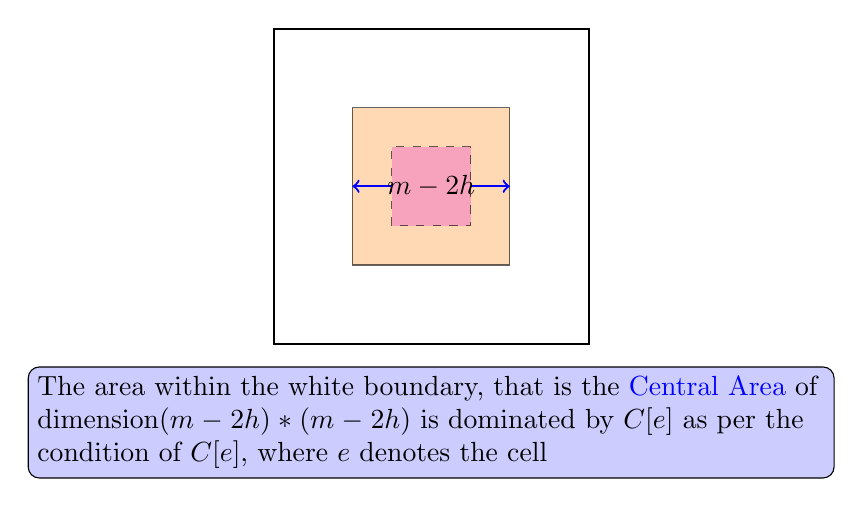
\begin{tikzpicture}

    % Square in the middle
    \draw[thick] (1, 1) rectangle ++(4, 4);
    \draw[fill=orange!50, opacity = 0.6] (2, 2) rectangle ++(2, 2);
    \draw[dashed, fill=magenta!50, opacity = 0.6] (2.5, 2.5) rectangle ++(1, 1);

    \draw[->, blue, thick ] (2.5, 3) -- (2,3) ;
    \draw[->, blue, thick ] (3.5, 3) -- (4,3) ;
    \node at (3,3) {$m -2h$};

    \node[draw, fill=blue!20, text width=10cm, rounded corners] at (3, 0) {
    The area within the white boundary, that is the \textcolor{blue}{Central Area} of dimension\textbf{$ (m-2h) * (m-2h) $} is dominated by $C[e]$ as per the condition of $C[e]$, where $e$ denotes the cell  
    };
    
     

\end{tikzpicture}

\end{center}

\end{frame}

\begin{frame}{Lemma 4.7}

\begin{center}
    

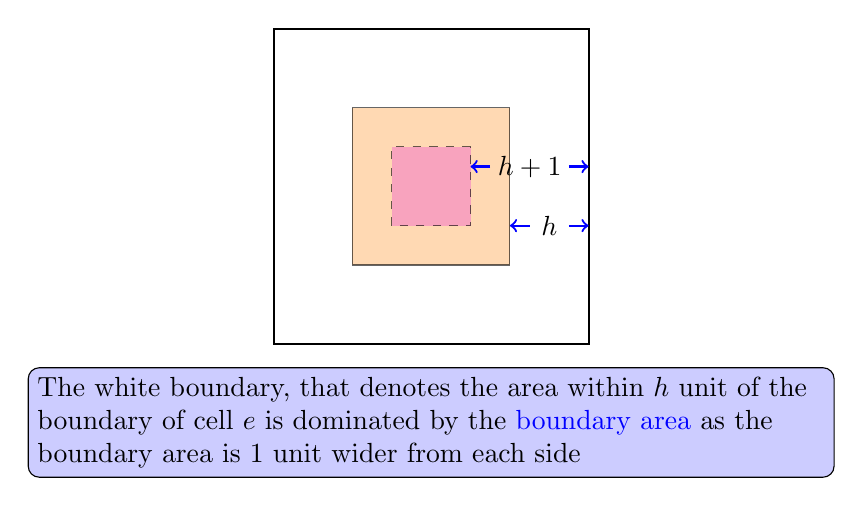
\begin{tikzpicture}

    % Square in the middle
    \draw[thick] (1, 1) rectangle ++(4, 4);
    \draw[fill=orange!50, opacity = 0.6] (2, 2) rectangle ++(2, 2);
    \draw[dashed, fill=magenta!50, opacity = 0.6] (2.5, 2.5) rectangle ++(1, 1);

    \draw[->, blue, thick ] (3.75,3.25) -- (3.5, 3.25) ;
    \draw[->, blue, thick ] (4.75,3.25)-- (5,3.25) ;
    \node at(4.25,3.25) {$h+1$};

    \draw[->, blue, thick ] (4.25,2.5)-- (4,2.5) ;
    \draw[->, blue, thick ] (4.75,2.5)-- (5,2.5) ;
    \node at(4.5,2.5) {$h$};
    
    \node[draw, fill=blue!20, text width=10cm, rounded corners] at (3, 0) {
    The white boundary, that denotes the area within \textbf{$h$} unit of the boundary of cell $e$ is dominated by the \textcolor{blue}{boundary area} as the boundary area is 1 unit wider from each side};

\end{tikzpicture}

\end{center}

\end{frame}

\begin{frame}{Lemma 4.7}

\begin{center}
    

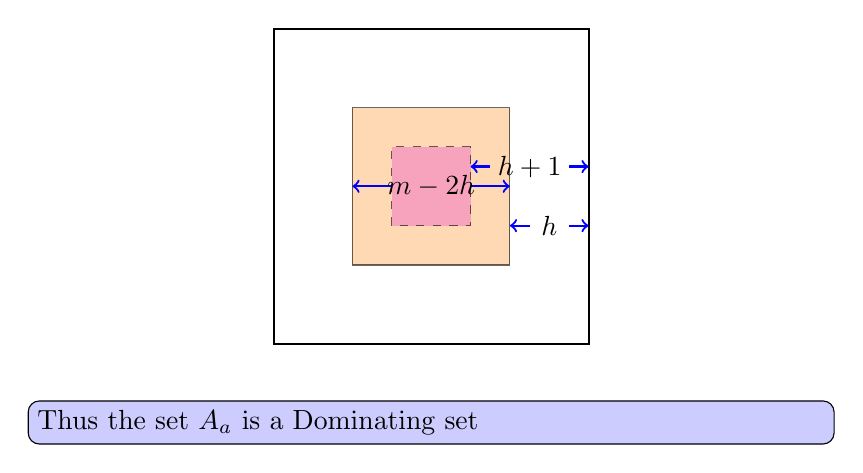
\begin{tikzpicture}

    % Square in the middle
    \draw[thick] (1, 1) rectangle ++(4, 4);
    \draw[fill=orange!50, opacity = 0.6] (2, 2) rectangle ++(2, 2);
    \draw[dashed, fill=magenta!50, opacity = 0.6] (2.5, 2.5) rectangle ++(1, 1);

    \draw[->, blue, thick ] (3.75,3.25) -- (3.5, 3.25) ;
    \draw[->, blue, thick ] (4.75,3.25)-- (5,3.25) ;
    \node at(4.25,3.25) {$h+1$};

    \draw[->, blue, thick ] (4.25,2.5)-- (4,2.5) ;
    \draw[->, blue, thick ] (4.75,2.5)-- (5,2.5) ;
    \node at(4.5,2.5) {$h$};

    \draw[->, blue, thick ] (2.5, 3) -- (2,3) ;
    \draw[->, blue, thick ] (3.5, 3) -- (4,3) ;
    \node at (3,3) {$m -2h$};
    
    \node[draw, fill=blue!20, text width=10cm, rounded corners] at (3, 0) {
    Thus the set $A_a$ is a Dominating set};

\end{tikzpicture}

\end{center}

\end{frame}

\begin{frame}{Lemma 4.7}

\begin{center}
    

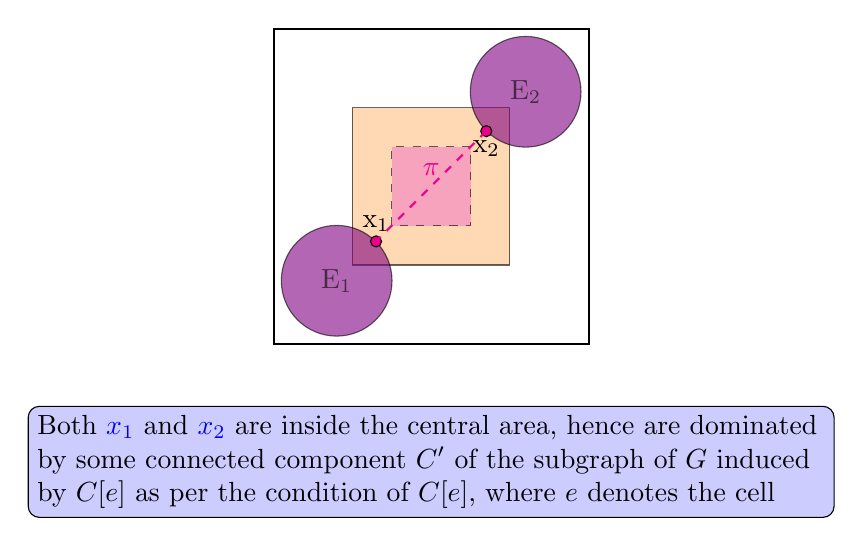
\begin{tikzpicture}

    % Square in the middle
    \draw[thick] (1, 1) rectangle ++(4, 4);
    \draw[fill=orange!50, opacity = 0.6] (2, 2) rectangle ++(2, 2);
    \draw[dashed, fill=magenta!50, opacity = 0.6] (2.5, 2.5) rectangle ++(1, 1);

    \filldraw[fill=violet, opacity = 0.6] (1.8, 1.8) circle (20pt) node {E$_1$};
    \filldraw[fill=violet, opacity = 0.6] (4.2, 4.2) circle (20pt) node {E$_2$};

    \filldraw[fill=magenta] (3.7, 3.7) circle (2pt) node[below] {x$_2$};
    \filldraw[fill=magenta] (2.3, 2.3) circle (2pt) node[above] {x$_1$};

    \draw[thick, dashed, magenta] (3.7, 3.7) -- (2.3, 2.3) node[above, midway]{\textbf{$\pi$}};

    \node[draw, fill=blue!20, text width=10cm, rounded corners] at (3, -0.5) {
    Both \textcolor{blue}{$x_1$} and \textcolor{blue}{$x_2$} are inside the central area, hence are dominated by some connected component $C^\prime$ of the subgraph of $G$ induced by $C[e]$ as per the condition of $C[e]$, where $e$ denotes the cell  
    };
    
     

\end{tikzpicture}

\end{center}

\end{frame}

\section{Algorithm 4.B is a PTAS}

\begin{frame}{Algorithm 4.B is a PTAS}

\begin{exampleblock}{Runtime of $C[e]$ computation for each cell $e$ in partition $P(a,a)$}

    \begin{equation}
        \sum_{e \in P(a,a)} n_e^{O(m^2)} \le \left ( \sum_{e \in P(a,a)} n_e \right ) ^{O(m^2)} = n^{O(m^2)} 
    \end{equation}
    

\end{exampleblock}

\begin{exampleblock}{Runtime of algorithm 4.B}

    \For {$a \gets 0$ to $m - 1$} \textcolor{red}{ $\xrightarrow{} O(m)$ } 

    \vspace{0.5em}
    
        \hspace{4em} $D_a \gets \{v \in D \mid v \text{ lies in the boundary area of } P(a, a)\} \textcolor{red}{  \xrightarrow{} O(n) }$ 

    \vspace{0.5em}
        
        \hspace{4em} $Compute \bigcup\limits_{e \in P(a,a)} C[e] \textcolor{red}{  \xrightarrow{} n^{O(m^2)} }$

    \vspace{2em}

        $ Runtime = \textcolor{red}{ O(mn) + m \cdot n^{O(m^2)} } $
    

\end{exampleblock}

\end{frame}

\section{Theorem 4.8}


\begin{frame}

    \begin{block}{Theorem 4.8}

        Output $A_a^*$ of algorithm $4.B$ is a $(1 + \varepsilon)-approximation$ for CDS-UDG with computation time $ n^{O(1/{\varepsilon^2})} $.
        
    \end{block}
    
\end{frame}

\begin{frame}{Theorem 4.8}

    \begin{center}
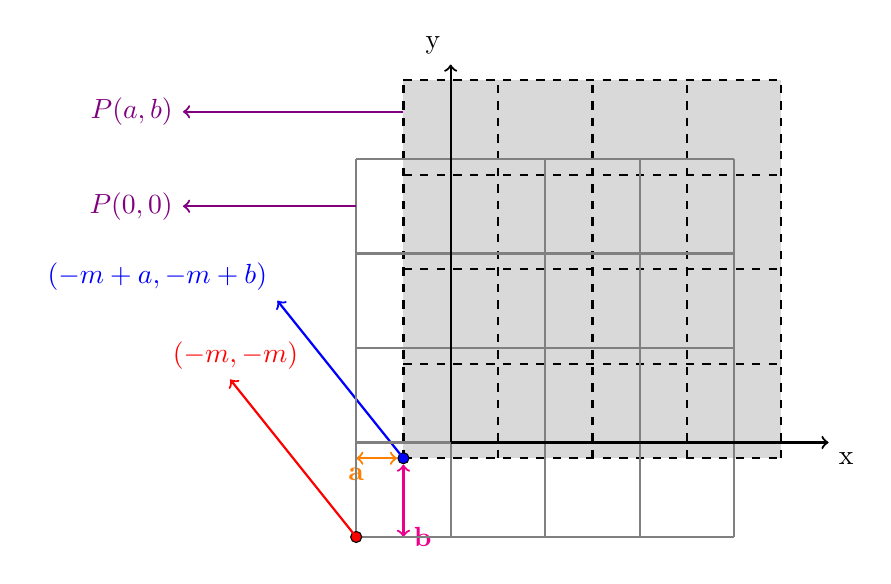
\begin{tikzpicture}[scale=0.4]

    \fill[gray!30] (0,0) rectangle (12,12);

   

    % Second Grid (dashed), positioned 2 units left and 3 units below
   
    \draw[step=3cm,black,dashed, thick] (0,0) grid (12,12);
    \filldraw[fill=blue] circle (5pt) ;
    \draw[orange, <->, thick] (-0.2, 0) -- (-1.5, 0) node[below] {\textbf{a}};
    \draw[magenta, <->, thick] (0, -0.2) -- (0, -2.5) node[right] {\textbf{b}};
    \draw[blue, ->, thick] (0, 0) -- (-4, 5) node[anchor=south east] {\textbf{ $(-m+a,-m+b)$}};

    
    

    \begin{scope}[xshift=-1.5cm, yshift=-2.5cm]
        \draw[step=3cm,gray, thick] (0,0) grid (12,12);
        \filldraw[fill=red] circle (5pt) ;
        \draw[red, ->, thick] (0, 0) -- (-4, 5) node[above] {\textbf{ $(-m,-m)$}};
        \draw[thick,->,black] (3,3) -- (15,3) node[anchor=north west] {x};
        \draw[thick,->,black] (3,3) -- (3,15) node[anchor=south east] {y};
    \end{scope}

    \draw[thick,->,violet] (0,11) -- (-7,11) node[left] {$P(a,b)$};
    \draw[thick,->,violet] (-1.5,8) -- (-7,8) node[left] {$P(0,0)$};

\end{tikzpicture}
\end{center}

%\draw[blue, ->, thick] (13.5, 13.5) -- (16, 15) node[right] {\textbf{\textit{\huge $\frac{1}{\sqrt{2}} \times \frac{1}{\sqrt{2}}$}}};
    
\end{frame}

\begin{frame}{Theorem 4.8 contd...}

    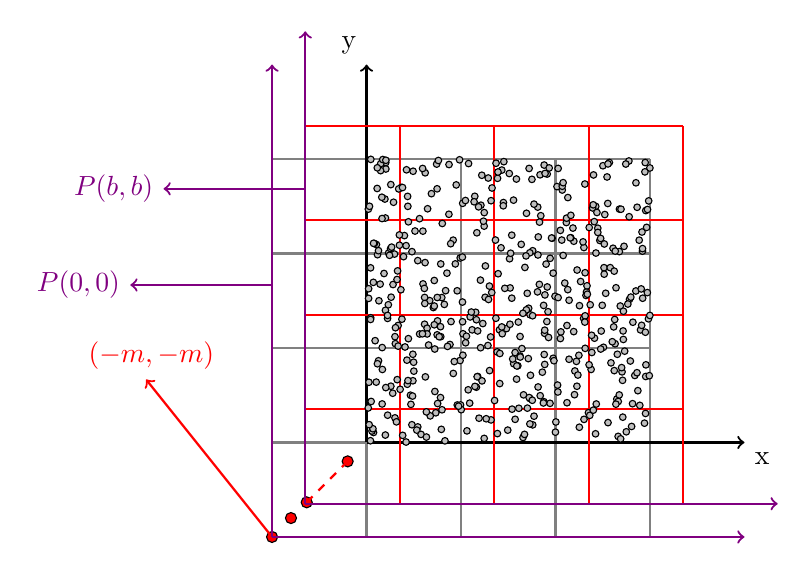
\begin{tikzpicture}[scale=0.4]

    % Draw the grid
    \draw[step=3cm,gray, thick] (0,0) grid (12,12);
    \filldraw[fill=red] circle (5pt) ;
    \filldraw[fill=red] (0.6,0.6) circle (5pt) ;

    \filldraw[fill=red] (1.1,1.1) circle (5pt) ;

    \filldraw[fill=red] (2.4,2.4) circle (5pt) ;

    \draw[red, dashed, thick] (1.1, 1.1) -- (2.4, 2.4);
        
    \draw[red, ->, thick] (0, 0) -- (-4, 5) node[above] {\textbf{ $(-m,-m)$}};
    \draw[thick,->,black] (3,3) -- (15,3) node[anchor=north west] {x};
    \draw[thick,->,black] (3,3) -- (3,15) node[anchor=south east] {y};

    \draw[thick,->,violet] (0,0) -- (15,0) ;
    \draw[thick,->,violet] (0,0) -- (0,15) ;

    

    \begin{scope}[xshift = 30, yshift = 30]
    
    \draw[step=3cm, red, thick] (0,0) grid (12,12);
  
    \draw[thick,->,violet] (0,0) -- (15,0) ;
    \draw[thick,->,violet] (0,0) -- (0,15) ;
    \draw[thick,->,violet] (0,10) -- (-4.5,10) node[left] {$P(b,b)$};

    \end{scope}

    \draw[thick,->,violet] (0,8) -- (-4.5,8) node[left] {$P(0,0)$};

    

    % Seed for randomness
    \pgfmathsetseed{42}  % Set seed for reproducibility

    % Generate 10 random points within the grid
    \foreach \i in {1,...,500} {
        \pgfmathsetmacro{\x}{3 + rnd*9}
        \pgfmathsetmacro{\y}{3 + rnd*9}
        \filldraw[fill=gray!50] (\x,\y) circle (3pt); % Draw a red point at random (x,y)
    }

\end{tikzpicture}
    
\end{frame}

\begin{frame}{Theorem 4.8 contd...}

    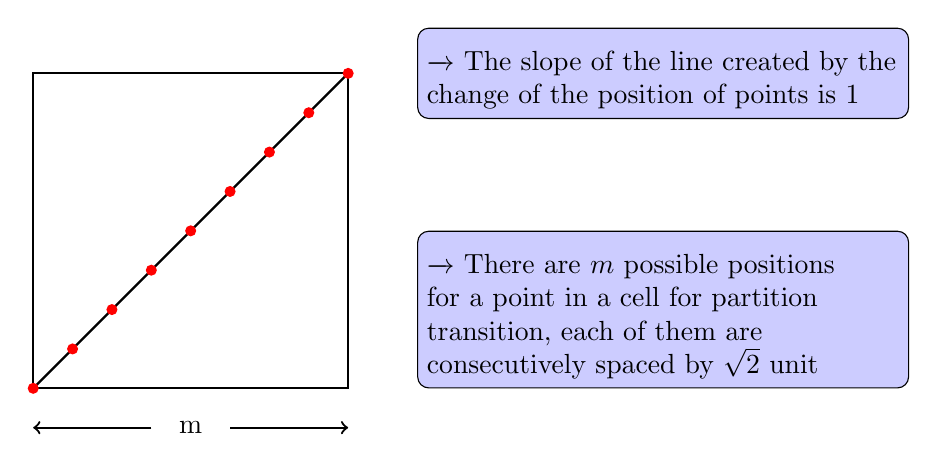
\begin{tikzpicture}

    % Draw the square
    \draw[thick] (0, 0) rectangle (4, 4);
    
    % Draw the diagonal
    \draw[thick] (0, 0) -- (4, 4);

    \draw[thick, ->] (1.5,-0.5) -- (0, -0.5); 
    \draw[thick, ->] (2.5, -0.5) -- (4, -0.5);
    \node at (2,-0.5) {m};

    % Add red points at regular intervals along the diagonal
    \foreach \i in {0, 0.5, 1, 1.5, 2, 2.5, 3, 3.5, 4} {
        \fill[red] (\i, \i) circle (2pt);
    }

    \node[draw, fill=blue!20, text width=6cm, rounded corners] at (8, 4) {

        $\xrightarrow{} $ The slope of the line created by the change of the position of points is 1
    };

    \node[draw, fill=blue!20, text width=6cm, rounded corners] at (8, 1) {
    
        $\xrightarrow{} $ There are $m$ possible positions for a point in a cell for partition transition, each of them are consecutively spaced by $\sqrt{2}$ unit
    };   

     
    

\end{tikzpicture}
    
\end{frame}

\begin{frame}{Theorem 4.8 contd...}

    \begin{center}
    

    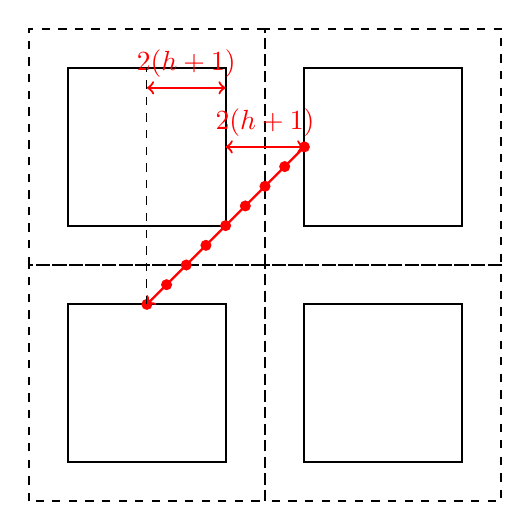
\begin{tikzpicture}

        \draw[thick, dashed] (0, 0) rectangle (3, 3);

        \draw[thick, dashed] (0, 3) rectangle (3, 6);

        \draw[thick, dashed] (-3, 0) rectangle (0, 3);

        \draw[thick, dashed] (-3, 3) rectangle (0, 6);


        \draw[thick] (0.5, 0.5) rectangle (2.5, 2.5);

        \draw[thick] (0.5, 3.5) rectangle (2.5, 5.5);

        \draw[thick] (-2.5, 0.5) rectangle (-0.5, 2.5);

        \draw[thick] (-2.5, 3.5) rectangle (-0.5, 5.5);

        \foreach \i in { 0, 0.25, 0.5,0.75, 1,1.25, 1.5,1.75, 2 } {
            \fill[red] (-1.5 + \i, 2.5 + \i) circle (2pt);
        }

        \draw[->, thick, red] (0.5, 4.5) -- (-1.5, 2.5)  ;

        \draw[<->, thick,red] (-0.5, 5.25) -- (-1.5, 5.25) node[above, midway]{$2(h+1)$} ;

        \draw[<->, thick,red] (0.5, 4.5) -- (-0.5, 4.5) node[above, midway]{$2(h+1)$};

        \draw[ thin,dashed] (-1.5, 2.5) -- (-1.5, 5.5);

    

    \end{tikzpicture}

\end{center}
    
\end{frame}

\begin{frame}{Theorem 4.8 contd...}


\begin{exampleblock}{Claim}

    \begin{equation}
        6 \cdot \lvert D_b^* \rvert + \lvert D_b \rvert \le \varepsilon \cdot \lvert D^* \rvert        
    \end{equation}

% \begin{exampleblock}{Runtime of $C[e]$ computation for each cell $e$ in partition $P(a,a)$}

%     \begin{equation}
%         \sum_{e \in P(a,a)} n_e^{O(m^2)} \le (\sum_{e \in P(a,a)} n_e) ^{O(m^2)} = n^{O(m^2)} 
%     \end{equation}
    

\end{exampleblock}

\begin{exampleblock}{}

    For any vertex $v$ in $D^*$, it belongs to at most $4(h + 1)$ of the sets
    $D_0^*, D^*_1,...,D^*_{m - 1}$. Therefore, by the pigeonhole principle, we have

    \begin{equation}    
        \displaystyle \sum_{a=0}^{m-1} \lvert D_a^* \rvert \le 4( h+1 )\lvert D^* \rvert         
    \end{equation}

    For any vertex $v$ in $D$, it belongs to at most $4(h + 1)$ of the sets
    $D_0, D_1,...,D_{m - 1}$. Therefore, by the pigeonhole principle, we have

    \begin{equation}    
        \displaystyle \sum_{a=0}^{m-1} \lvert D_a \rvert \le 4( h+1 )\lvert D \rvert \le 16( h+1 )\lvert D^* \rvert         
    \end{equation}
    

\end{exampleblock}

\end{frame}

\begin{frame}{Theorem 4.8 contd...}


\begin{exampleblock}{Adding $6*(3)$ and $(4)$}

    \begin{equation}
            6 \cdot \displaystyle \sum_{a=0}^{m-1} \lvert D_a^* \rvert + \displaystyle \sum_{a=0}^{m-1} \lvert D_a \rvert \le 40( h+1 )\lvert D^* \rvert   
    \end{equation}

% \begin{exampleblock}{Runtime of $C[e]$ computation for each cell $e$ in partition $P(a,a)$}

%     \begin{equation}
%         \sum_{e \in P(a,a)} n_e^{O(m^2)} \le (\sum_{e \in P(a,a)} n_e) ^{O(m^2)} = n^{O(m^2)} 
%     \end{equation}
    

\end{exampleblock}

\begin{exampleblock}{}

    Therefore, again applying the pigeonhole principle, there must exist an integer $b \hspace{0.5em} \epsilon \hspace{0.5em} \{0, 1,...,m - 1\}$ such that,

    \begin{equation}
            6 \cdot \lvert D_b^* \rvert + \lvert D_b \rvert \le \frac{40( h+1 )}{m}\lvert D^* \rvert  \le \varepsilon \cdot \lvert D^* \rvert
    \end{equation}

% \begin{exampleblock}{Runtime of $C[e]$ computation for each cell $e$ in partition $P(a,a)$}

%     \begin{equation}
%         \sum_{e \in P(a,a)} n_e^{O(m^2)} \le (\sum_{e \in P(a,a)} n_e) ^{O(m^2)} = n^{O(m^2)} 
%     \end{equation}
    

\end{exampleblock}



\end{frame}

\begin{frame}{Theorem 4.8 contd...}

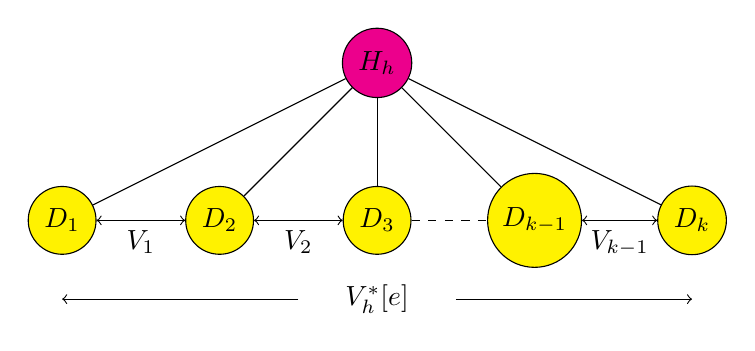
\begin{tikzpicture}

% Define the central node
\node[draw, circle, fill = magenta, minimum size=20pt] (H) at (0, 2) {$H_h$};

% Define the servant nodes along the x-axis
\node[draw, circle, fill = yellow] (node1) at (-4, 0) {$D_1$};
\node[draw, circle, fill = yellow] (node2) at (-2, 0) {$D_2$};
\node[draw, circle, fill = yellow] (node3) at (0, 0) {$D_3$};
\node[draw, circle, fill = yellow] (node1k) at (2, 0) {$D_{k-1}$};
\node[draw, circle, fill = yellow] (nodek) at (4, 0) {$D_{k}$};

% Connect servant nodes to the central node
\draw (H) -- (node1);
\draw (H) -- (node2);
\draw (H) -- (node3);
\draw (H) -- (node1k);
\draw (H) -- (nodek);

% Connect servant nodes to each other
\draw[<->] (node1) -- node[midway, below] {$V_1$} (node2) ;
\draw[<->] (node2) -- node[midway, below] {$V_2$} (node3) ;
\draw[dashed] (node3) -- (node1k);
\draw[<->] (node1k) -- node[midway, below] {$V_{k-1}$} (nodek);

\draw [->, ] (-1,-1) -- (-4,-1);

\draw [->, ] (1,-1) -- (4,-1);

\node at (0,-1){$V^*_h[e]$};

\end{tikzpicture}

\end{frame}

\begin{frame}{Theorem 4.8 contd...}


{\tiny

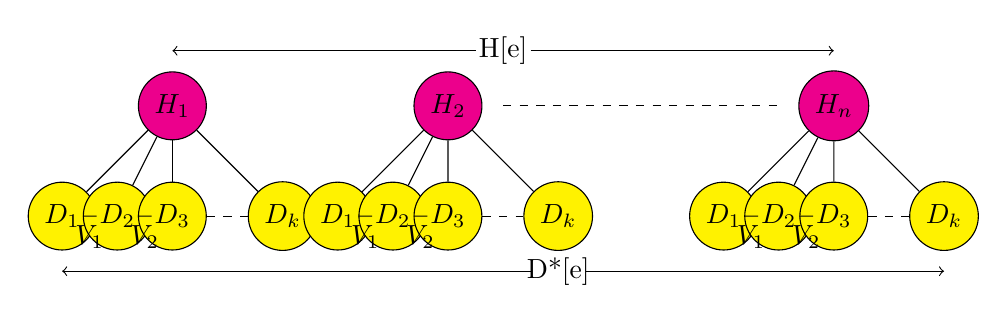
\begin{tikzpicture}[scale=0.7, every node/.style={minimum size=5pt}]

% Define the central nodes
\node[draw, circle, fill=magenta, minimum size=5pt] (H1) at (0, 2) {$H_1$};
\node[draw, circle, fill=yellow] (node1_1) at (-2, 0) {$D_1$};
\node[draw, circle, fill=yellow] (node2_1) at (-1, 0) {$D_2$};
\node[draw, circle, fill=yellow] (node3_1) at (0, 0) {$D_3$};
% \node[draw, circle, fill=yellow] (node4_1) at (1.5, 0) {$D_{k-1}$};
\node[draw, circle, fill=yellow] (node5_1) at (2, 0) {$D_k$};
\draw (H1) -- (node1_1) -- node[midway, below] {$V_1$} (node2_1);
\draw (H1) -- (node2_1) -- node[midway, below] {$V_2$} (node3_1);
\draw (H1) -- (node3_1) ;
\draw[dashed] (node3_1) -- (node5_1);
% \draw (H1) -- (node4_1) -- node[midway, below] {$V_{k-1}$} (node5_1);
\draw (H1) -- (node5_1);

% Second star network (shifted by 12 units to the right)
\node[draw, circle, fill=magenta, minimum size=5pt] (H2) at (5, 2) {$H_2$};
\node[draw, circle, fill=yellow] (node1_2) at (3, 0) {$D_1$};
\node[draw, circle, fill=yellow] (node2_2) at (4, 0) {$D_2$};
\node[draw, circle, fill=yellow] (node3_2) at (5, 0) {$D_3$};
% \node[draw, circle, fill=yellow] (node4_2) at (7.5, 0) {$D_{k-1}$};
\node[draw, circle, fill=yellow] (node5_2) at (7, 0) {$D_k$};
\draw (H2) -- (node1_2) -- node[midway, below] {$V_1$} (node2_2);
\draw (H2) -- (node2_2) -- node[midway, below] {$V_2$} (node3_2);
\draw (H2) -- (node3_2);
\draw[dashed] (node3_2) -- (node5_2);
% \draw (H2) -- (node4_2) -- node[midway, below] {$V_{k-1}$} (node5_2);
\draw (H2) -- (node5_2);

% Third star network (shifted by 24 units to the right)
\node[draw, circle, fill=magenta, minimum size=5pt] (H3) at (12, 2) {$H_n$};
\node[draw, circle, fill=yellow] (node1_3) at (10, 0) {$D_1$};
\node[draw, circle, fill=yellow] (node2_3) at (11, 0) {$D_2$};
\node[draw, circle, fill=yellow] (node3_3) at (12, 0) {$D_3$};
% \node[draw, circle, fill=yellow] (node4_3) at (13.5, 0) {$D_{k-1}$};
\node[draw, circle, fill=yellow] (node5_3) at (14, 0) {$D_k$};
\draw (H3) -- (node1_3) -- node[midway, below] {$V_1$} (node2_3);
\draw (H3) -- (node2_3) -- node[midway, below] {$V_2$} (node3_3);
\draw (H3) -- (node3_3) ;
\draw[dashed] (node3_3) -- (node5_3);
% \draw (H3) -- (node4_3) -- node[midway, below] {$V_{k-1}$} (node5_3);
\draw (H3) -- (node5_3);

\draw [dashed] (6,2) -- (11,2);

\draw [->, ] (6.5,-1) -- (-2,-1);

\draw [->, ] (7.5,-1) -- (14,-1);

\node at (7,-1){D*[e]};

\draw [->, ] (5.5,3) -- (0,3);

\draw [->, ] (6.5,3) -- (12,3);

\node at (6,3){H[e]};


\end{tikzpicture}

}


\end{frame}

\begin{frame}{Theorem 4.8 contd...}




\begin{exampleblock}{}

    For any cell $e$ that has $n$ connected components in central Area,

    \vspace{0.5em}
    
    $\lvert V^*[e] \rvert = \displaystyle \sum_{h=0}^{n} \lvert V^*_h[e] \rvert \le 2(k -1) n$ 

    \vspace{0.5em}

    $\lvert D^\prime[e] \rvert = \lvert D^*[e] \rvert + \lvert V^*[e] \rvert \le \lvert D^*[e] \rvert + 2(k -1) n$ 

    \vspace{1em}

    We define $D^\prime$ for some $b \epsilon \{0,1,2,..., m -1\} ,$

    \vspace{0.5em}

    $D^\prime = D_b \cup \left( \bigcup\limits_{e \in P(b,b)} D^\prime[e] \right)$

    \vspace{0.5em}

   Clearly for each connected component $H$ of central area $G_c[e]$, $D^\prime$ has a connected component dominating $H$. However, not necessarily with minimum number of vertices. 

    \begin{equation}    
          \lvert A_b \rvert \le \lvert D^\prime \rvert           
    \end{equation}
    

\end{exampleblock}

\end{frame}

\addtocounter{framenumber}{3}

% \begin{frame}{Theorem 4.8 contd...}

% 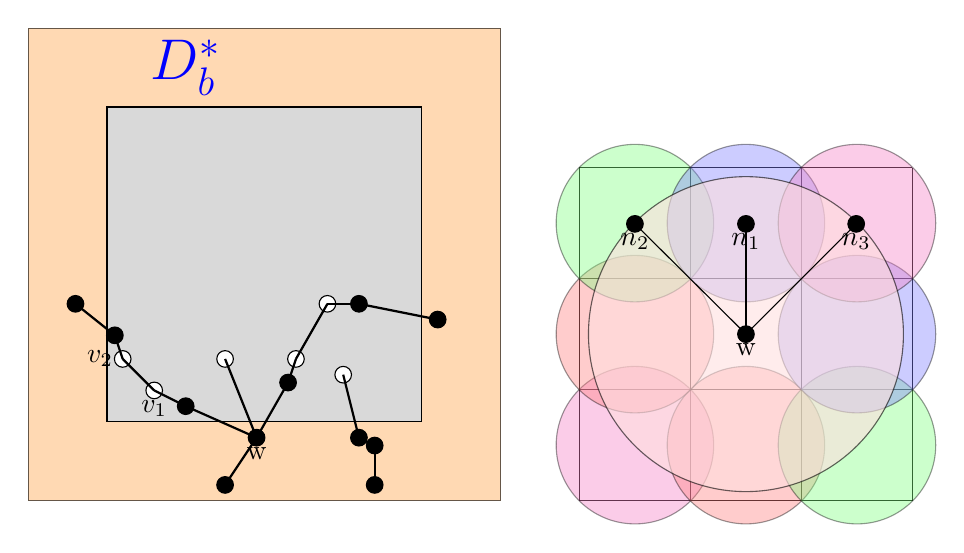
\begin{tikzpicture}

    % Square in the middle
    
    \draw[ fill=orange!50, opacity=0.6] (2, 2) rectangle ++(6, 6);
    \draw[ fill=gray!30] (3, 3) rectangle ++(4, 4);

    

    \coordinate (v6) at (4.9, 2.8);

    \filldraw[fill=black] (v6) circle (3pt) node[below]{w};

    \coordinate (v72) at (4.5, 2.2);

    \filldraw[fill=black] (v72) circle (3pt);

    \coordinate (v9b) at (6.2, 2.8);

    \filldraw[fill=black] (v9b) circle (3pt);

    \coordinate (v9c) at (6.4, 2.7);

    \filldraw[fill=black] (v9c) circle (3pt);

    \coordinate (v9d) at (6.4, 2.2);

    \filldraw[fill=black] (v9d) circle (3pt);

    \coordinate (v92) at (7.2, 4.3);

    \filldraw[fill=black] (v92) circle (3pt);

    \coordinate (v5) at (4.5, 3.8);

    \filldraw[fill=white] (v5) circle (3pt);

    \coordinate (v71) at (5.3, 3.5);

    \filldraw[fill=black] (v71) circle (3pt);

    \coordinate (v73) at (5.4, 3.8);

    \filldraw[fill=white] (v73) circle (3pt);

    \coordinate (v10) at (4, 3.2);

    \filldraw[fill=black] (v10) circle (3pt);

    \coordinate (v11) at (3.6, 3.4);

    \filldraw[fill=white] (v11) circle (3pt) node[below]{$v_1$};

    \coordinate (v12) at (3.2, 3.8);

    \filldraw[fill=white] (v12) circle (3pt) node[left]{$v_2$};

    \coordinate (v13) at (3.1, 4.1);

    \filldraw[fill=black] (v13) circle (3pt) ;

    \coordinate (v14) at (2.6, 4.5);

    \filldraw[fill=black] (v14) circle (3pt) ;
    

    

    

    

    \coordinate (v9a) at (6, 3.6);

    \filldraw[fill=white] (v9a) circle (3pt);

    \coordinate (v91) at (6.2, 4.5);

    \filldraw[fill=black] (v91) circle (3pt);

    \coordinate (v93) at (5.8, 4.5);

    \filldraw[fill=white] (v93) circle (3pt);

    

    

    

   \node at (4,7.5) {\huge{\textcolor{blue}{$D^*_b$}}};



    
    \draw [thick, black](v5) -- (v6);
    \draw [thick, black](v6) -- (v71);
    \draw [thick, black](v91) -- (v92);
    \draw [thick, black](v9a) -- (v9b);

   
    


    \draw [thick, black](v6) -- (v72);
    \draw [thick, black](v9b) -- (v9c);
    \draw [thick, black](v9c) -- (v9d);
    \draw [thick, black](v91) -- (v93);
    \draw [thick, black](v71) -- (v73);
    \draw [thick, black](v10) -- (v6);
    \draw [thick, black](v10) -- (v11);
    \draw [thick, black](v12) -- (v11);
    \draw [thick, black](v12) -- (v13);
    \draw [thick, black](v13) -- (v14);
    \draw [thick, black](v73) -- (v93);


    \begin{scope}[xshift= 9cm, yshift = 2cm]

        \draw[step = 1.41] (0, 0) grid (4.23, 4.23);
        \draw[fill = magenta!50, opacity = 0.4] (0.705, 0.705) circle (1);
        \draw[fill = red!50, opacity = 0.4] (2.115, 0.705) circle (1);
        \draw[fill = green!50, opacity = 0.4] (3.525, 0.705) circle (1);
        \draw[fill = red!50, opacity = 0.4] ( 0.705, 2.115) circle (1);
        \draw[fill = green!50, opacity = 0.4] ( 0.705, 3.525) circle (1);
        \draw[fill = blue!50, opacity = 0.4] ( 2.115, 3.525) circle (1);
        \draw[fill = blue!50, opacity = 0.4] ( 3.525, 2.115) circle (1);
        \draw[fill = magenta!50, opacity = 0.4] ( 3.525, 3.525) circle (1);
        \draw[fill = pink!50, opacity = 0.6] ( 2.115, 2.115) circle (2);

        \draw[fill = black] ( 2.115, 2.115) circle (3pt) node[below]{w};
        \draw[fill = black] ( 2.115, 3.515) circle (3pt);
        \draw[fill = black] ( 0.705, 3.515) circle (3pt);
        \draw[fill = black] ( 3.515, 3.515) circle (3pt);

        \draw[] ( 2.115, 2.115) -- ( 2.115, 3.515) node[below]{$n_1$};
        \draw[] ( 2.115, 2.115) -- ( 0.705, 3.515) node[below]{$n_2$};
        \draw[] ( 2.115, 2.115) -- ( 3.515, 3.515) node[below]{$n_3$};
        

        
    \end{scope}

    


    

\end{tikzpicture}



% \end{frame}

\end{document}


